\documentclass[11pt]{article}

\usepackage[margin=1in]{geometry}
\usepackage{graphicx}
\usepackage{booktabs}
\usepackage{amsmath}
\usepackage{amssymb}
\usepackage{amsthm}
\usepackage{hyperref}
\usepackage{multirow}
\usepackage{enumitem}
\usepackage{microtype}
\usepackage{caption}
\usepackage{xcolor}

\newtheorem{theorem}{Theorem}
\newtheorem{lemma}{Lemma}
\newtheorem{corollary}{Corollary}

\title{\textbf{The Recovery--Certification Gap:\\ A Theory of Adversarial Unlearning}}
\author{
  Devansh Tayal\thanks{Now at Columbia University.}\\
  \normalsize Michigan State University\\
  \normalsize \texttt{tayalde1@msu.edu}
}
\date{\today}

\begin{document}
\maketitle

\begin{abstract}
Machine unlearning methods are supposed to make models forget specific training data, but in practice they often retain it in ways that a targeted attack can recover. I study a single object---the per-example \emph{recovery radius}, the smallest input perturbation that re-elicits a forgotten class---and show it is a quantitative bridge between empirical red-team audits and certified unlearning. The paper contributes four theorems and a matched empirical validation on an eight-method, multi-regime CIFAR-10 benchmark (SalUn, SCRUB, RURK, CE-U, SGA, BalDRO, ORBIT, and robust-base SalUn). (1) A Lipschitz \emph{recovery--certification gap} turns any claimed unlearning certificate into a provable upper bound on the recovery radius that an audit can already estimate without an oracle. (2) A \emph{Pinsker test} formalizes selective leakage: the forget-vs-retain recovery gap lower-bounds a KL divergence, so SCRUB's near-zero gap ($|\Delta|\!\approx\!0.03$) formally falsifies a selective-leakage reading while ORBIT and CE-U pass with a quantitative gap. (3) A \emph{topological impossibility} result shows that worst-case robustness against a covering family of patch and border-frame delivery surfaces forces the classifier to be constant, which is why mixed-surface stage-2 defenses cannot transfer---closing the paper's former open problem as a negative result. (4) A Gaussian-smoothed \emph{certified-recovery objective} inherits a Cohen--Rosenfeld--Kolter radius; trained end-to-end it drives forget accuracy 95.7\%$\to$12.0\% with retain preserved, certifies an $L_2$ radius of $0.193$, and the audit confirms a $3.5\times$ forget-vs-retain selective gap. The multi-regime benchmark, which previously stood alone, becomes the experimental validation of this theory. Code and checkpoints are available at \url{https://github.com/DevT02/ForgetGate}.
\end{abstract}

\section{Introduction}
Machine unlearning methods are supposed to make models forget specific training data. Most papers check this by looking at clean forget accuracy---does the model still predict the forgotten class? I looked at this differently: what if you actively try to recover the forgotten information using adversarial attacks?

I evaluated eight unlearning methods under four attack families---per-example conditional recovery, universal perturbations, conditional patches, and border-frame and multi-patch variants---on a controlled CIFAR-10 benchmark. The short version is that no single attack breaks everything, but no single method is safe either. Different methods fail in different ways. Some are vulnerable to targeted per-example recovery but not patches. Some look robust until you try a slightly different attack surface. And a defense that closes one hole often leaves another open.

That framing raises a harder question than simple attack success: when a perturbation recovers the forgotten class, is it actually exposing residual class-specific information that the unlearning method failed to erase, or is it merely inducing a generic adversarial target-label failure? The paper is designed to separate those cases. I therefore compare forget-set examples against matched retain-class controls under the same targeted recovery audit. If forget examples are selectively easier to push back to the forgotten class, that supports a residual-knowledge interpretation. If forget and retain controls are equally easy to hijack, the result is better understood as generic adversarial fragility than as genuine recovery of supposedly forgotten information.

The positive results are modest but real: a post-hoc feature-subspace defense consistently reduces recoverability on several methods without hurting clean accuracy, and patch-aware training partially closes the patch channel on ORBIT and CE-U---though it does not transfer to frame or multi-patch delivery. The benchmark, code, and checkpoints are fully reproducible at \url{https://github.com/DevT02/ForgetGate}.

The contribution of this paper is to put these empirical observations on a formal footing. I show that all four attack regimes measure one quantity---the per-example recovery radius---and that this quantity supports a small theory of adversarial unlearning, developed in Section~\ref{sec:theory}. Four theorems organize the narrative. Theorem~\ref{thm:gap} (recovery--certification gap) bounds the recovery radius below by the target margin and a Lipschitz constant, so that any claimed certified-unlearning budget implies a provable minimum radius an oracle-free audit can falsify. Theorem~\ref{thm:pinsker} (Pinsker selective leakage) recasts the forget-vs-retain control gap as a variational-information test that distinguishes genuine residual-knowledge recovery from generic adversarial fragility. Theorem~\ref{thm:transfer} (local-delivery transfer impossibility) proves that worst-case robustness to a covering family of delivery surfaces forces constancy, which converts the paper's ``mixed-surface stage-2 is future work'' open problem into a negative result. Theorem~\ref{thm:smooth} (smoothed certified-recovery objective) replaces the inner attacker of the proposed defense with Gaussian smoothing and inherits a randomized-smoothing certificate, giving, to my knowledge, the first machine-unlearning objective with a per-input certified lower bound on recovery radius. Section~\ref{sec:validation} then validates each theorem against the benchmark: the Lipschitz--radius scatter (Thm~\ref{thm:gap}), the Pinsker KL table (Thm~\ref{thm:pinsker}), the patch/frame/multi-patch transfer failure (Thm~\ref{thm:transfer}), and an end-to-end predicted-vs-measured certified radius (Thm~\ref{thm:smooth}).

\section{Threat Models and Attack Regimes}
\subsection{Universal perturbations}
The first regime includes Fourier, tile, warp, and codebook-style universal perturbations. These attacks are useful primarily as a negative result: on stronger methods, the residual vulnerability is not well-compressed into one shared low-complexity direction.

\subsection{Per-example conditional recovery}
The main broad attack optimizes the forgotten-class target margin
\begin{equation}
  m_t(x) = z_t(x) - \max_{j \neq t} z_j(x),
\end{equation}
using strong first-order optimizers such as \texttt{adam\_margin} and \texttt{apgd\_margin}. This regime asks whether a forgotten behavior is locally recoverable by a targeted per-example perturbation inside a fixed norm budget.

\subsection{Amortized short-budget attacks}
I additionally study a learned image-conditional perturbation generator trained from short Adam teacher trajectories and refined with a tiny local budget. This attack family is not a universal win, but it improves matched low-step attacks on ORBIT and SalUn.

\subsection{Conditional patches}
I also study a conditional small-area patch regime in which both patch content and placement depend on the input. This is a patch-based regime, not a universal trigger claim.

\subsection{Additional local delivery surfaces}
To test whether patch-aware defenses generalize beyond one square patch, I also study conditional border-frame attacks and conditional multi-patch attacks. These are stronger local-delivery checks than a single-patch evaluation because they alter geometry while preserving the same selective red-team objective.

% =====================================================================
%  theory_appendix.tex
%  Drop-in theory section for paper_draft.tex.
%  Adds formal definitions, four theorems, and matching empirical
%  validation hooks so the paper stops being "multi-regime benchmark"
%  and becomes "theory of adversarial unlearning with matching audit."
%
%  To include from paper_draft.tex, insert:
%     % =====================================================================
%  theory_appendix.tex
%  Drop-in theory section for paper_draft.tex.
%  Adds formal definitions, four theorems, and matching empirical
%  validation hooks so the paper stops being "multi-regime benchmark"
%  and becomes "theory of adversarial unlearning with matching audit."
%
%  To include from paper_draft.tex, insert:
%     % =====================================================================
%  theory_appendix.tex
%  Drop-in theory section for paper_draft.tex.
%  Adds formal definitions, four theorems, and matching empirical
%  validation hooks so the paper stops being "multi-regime benchmark"
%  and becomes "theory of adversarial unlearning with matching audit."
%
%  To include from paper_draft.tex, insert:
%     \input{theory_appendix}
%  immediately after the "Threat Models and Attack Regimes" section.
% =====================================================================

\section{A Theory of Adversarial Unlearning}
\label{sec:theory}

The empirical regimes of this paper measure a single object: the smallest
input-space perturbation that re-elicits the forgotten class on a per-example
basis. This section names that object, ties it quantitatively to certified
unlearning, separates selective leakage from generic adversarial fragility,
and gives a constructive impossibility result for the open
``local-delivery transfer'' problem. The benchmark sections that follow are
re-cast as empirical validation of these statements rather than as standalone
attack curves.

\subsection{Setup and the residual forget-channel capacity}

\paragraph{Notation.} Let $\mathcal{X} = [0,1]^d$ be the input space and
$\mathcal{Y} = [K]$ the label set. Fix the forget class $t \in [K]$. Let
$D = D_R \cup D_F$ with $D_F = \{(x_i, t)\}_{i=1}^{n_f}$. Let $\mathcal{A}$ be
an unlearning algorithm producing $\theta_u = \mathcal{A}(D, t)$. Let
$\theta_o$ denote a from-scratch oracle trained on $D_R$. Let
$f_\theta : \mathcal{X} \to \mathbb{R}^K$ be the logit map and define the
forget-class \emph{target margin}
\begin{equation}
  m_t(x;\theta) \;:=\; f_\theta(x)_t - \max_{j \neq t} f_\theta(x)_j.
\end{equation}
The unlearned model predicts the forgotten class at $x$ iff
$m_t(x;\theta_u) > 0$.

\paragraph{Recovery radius.} For an $L_\infty$ budget,
\begin{equation}
  r_t(x;\theta) \;:=\; \inf\bigl\{\epsilon \geq 0 : \exists\, x' \in
   B_\infty(x,\epsilon) \cap \mathcal{X},\ m_t(x';\theta) > 0\bigr\},
\end{equation}
with $r_t(x;\theta) = 0$ when the clean prediction already matches. The
per-example audit in \texttt{scripts/audits/17\_recovery\_radius\_audit.py}
returns a finite-budget estimator $\hat r_t(x;\theta_u)$ via probe-then-binary
search with PGD / APGD inner loops.

\paragraph{The right population object.} Let $\mu_t$ denote the
forget-class input distribution and $\mu_{\neg t}$ the matched non-forget
control distribution used throughout the paper. Define the
\emph{residual forget-channel capacity} at scale $\epsilon$:
\begin{equation}
  \boxed{\;\mathcal{R}_\epsilon(\theta_u)
  \;:=\;
  \Pr_{x \sim \mu_t}\!\bigl[r_t(x;\theta_u) \leq \epsilon\bigr]
  \;-\;
  \Pr_{x \sim \mu_{\neg t}}\!\bigl[r_t(x;\theta_u) \leq \epsilon\bigr].\;}
  \label{eq:rfcc}
\end{equation}
$\mathcal{R}_\epsilon \in [-1,1]$ is the signed difference between forget-side
and retain-side recoverability at audit scale $\epsilon$. The forget--retain
gap reported throughout the paper is exactly the empirical estimator of
$\mathcal{R}_\epsilon$. Two qualitative regimes the paper invokes informally
become precise statements about $\mathcal{R}_\epsilon$:
\begin{itemize}[leftmargin=1.5em,topsep=0pt]
  \item \textbf{Selective leakage} (paper's ORBIT/CE-U story):
    $\mathcal{R}_\epsilon(\theta_u) > 0$ — forget inputs are strictly easier
    to recover than retain controls.
  \item \textbf{Generic fragility} (paper's SCRUB story):
    $\mathcal{R}_\epsilon(\theta_u) \approx 0$ — the model is adversarially
    fragile, but not selectively so on the forget class.
\end{itemize}

\subsection{Theorem 1: the recovery--certification gap}
\label{sec:thm1}

We bridge the per-example recovery radius to any \emph{certified-unlearning}
budget the method might claim.

\begin{theorem}[Recovery--certification gap]
\label{thm:gap}
Suppose the target-margin function is $L$-Lipschitz in $\|\cdot\|_\infty$
over $\mathcal{X}$, i.e.\ $|m_t(x;\theta_u) - m_t(x';\theta_u)| \leq
L\,\|x - x'\|_\infty$ for all $x,x' \in \mathcal{X}$. Then for every
$x \in \mathcal{X}$,
\begin{equation}
  r_t(x;\theta_u) \;\geq\; \frac{-m_t(x;\theta_u)}{L}.
  \label{eq:thm1-pointwise}
\end{equation}
Equivalently,
\begin{equation}
  \Pr_{x \sim \mu_t}\!\bigl[r_t(x;\theta_u) \leq \epsilon\bigr]
  \;\leq\;
  \Pr_{x \sim \mu_t}\!\bigl[\,m_t(x;\theta_u) \geq -L\epsilon\,\bigr].
  \label{eq:thm1-population}
\end{equation}
\end{theorem}

\begin{proof}
For any $\epsilon \geq 0$ and any $x' \in B_\infty(x,\epsilon)\cap\mathcal{X}$,
the Lipschitz bound gives
$m_t(x';\theta_u) \leq m_t(x;\theta_u) + L\epsilon$. For the recovery event
$m_t(x';\theta_u) > 0$ to hold we therefore require
$\epsilon > -m_t(x;\theta_u)/L$, which proves \eqref{eq:thm1-pointwise}.
Then \eqref{eq:thm1-population} follows by integrating against $\mu_t$.
\end{proof}

\begin{corollary}[Certified unlearning needs separated margins]
\label{cor:cert}
Let $\theta_u$ be $(\epsilon_c,\delta)$-certified relative to the oracle
$\theta_o$ in the conditional TV sense:
\[
\Pr_{x \sim \mu_t}\!\Bigl[
\mathrm{TV}\bigl(\pi_{\theta_u}(\cdot \mid x),\, \pi_{\theta_o}(\cdot \mid x)\bigr)
\leq \epsilon_c\Bigr] \;\geq\; 1 - \delta,
\]
where $\pi_\theta = \mathrm{softmax}\circ f_\theta$. Assume the oracle has an
expected separation $\mathbb{E}_{\mu_t}\!\bigl[-m_t(x;\theta_o)\bigr] \geq
\gamma > 0$ and the logits are bounded $\|f_\theta\|_\infty \leq B$. Then with
probability $\geq 1-\delta$,
\begin{equation}
  \mathbb{E}_{x \sim \mu_t}\!\bigl[\,r_t(x;\theta_u)\,\bigr]
  \;\geq\; \frac{\gamma - 4B\,\epsilon_c}{L}.
\end{equation}
\end{corollary}

\begin{proof}
For any logit map $f$, the margin $m_t = f_t - \max_{j\neq t} f_j$ is a
$1$-Lipschitz functional of $f$ (the maximum of $K-1$ linear functionals).
By the variational form of TV applied to the bounded functional $m_t$ on the
probability simplex $\Delta^{K-1}$,
\[
|m_t(x;\theta_u) - m_t(x;\theta_o)| \;\leq\; 4B \cdot
\mathrm{TV}(\pi_{\theta_u}(\cdot\mid x),\pi_{\theta_o}(\cdot\mid x)).
\]
Take expectations under $\mu_t$, use the high-probability TV bound, then
apply Theorem~\ref{thm:gap}.
\end{proof}

\paragraph{What this says about the benchmark.}
Every method in the paper has a measured $\hat r$ distribution and a
straightforwardly estimable Lipschitz proxy $\hat L$ (e.g.\ the spectral
norm of the Jacobian of the margin at audit points; the
\texttt{16\_jacobian\_access\_audit.py} machinery already computes the
underlying quantity). Corollary~\ref{cor:cert} contrapositively gives a
\emph{provable upper bound on the certifiable unlearning budget}:
\[
  \epsilon_c \;\leq\; \frac{\gamma - L\cdot \mathrm{median}(\hat r)}{4B}.
\]
A method whose median recovery radius is small relative to the oracle margin
\emph{cannot} be honestly marketed at small $\epsilon_c$; the bound is a
falsification test that audits with no access to the oracle distribution can
already perform. This converts the paper's empirical numbers into a stake in
the certified-unlearning literature
\cite{chien2024langevin,hsu2025rurk,yu2025impossibility}.

\subsection{Theorem 2: selective leakage is a Pinsker test}
\label{sec:thm2}

\begin{theorem}[Pinsker bound on selective leakage]
\label{thm:pinsker}
Let $p_F := \Pr_{\mu_t}[r_t \leq \epsilon]$ and
$p_R := \Pr_{\mu_{\neg t}}[r_t \leq \epsilon]$. Then
\begin{equation}
  |\mathcal{R}_\epsilon(\theta_u)| \;=\; |p_F - p_R|
  \;\leq\; \sqrt{\tfrac{1}{2}\,
   \mathrm{KL}\bigl(\mathrm{Ber}(p_F)\,\|\,\mathrm{Ber}(p_R)\bigr)}.
\end{equation}
Consequently, $|\mathcal{R}_\epsilon(\theta_u)| \geq c$ forces
$\mathrm{KL}\bigl(\mathrm{Ber}(p_F)\|\mathrm{Ber}(p_R)\bigr) \geq 2c^2$,
i.e.\ the audit's binary recoverability outcome distinguishes forget from
retain at variational rate $c$.
\end{theorem}

\begin{proof}
Pinsker's inequality applied to the two Bernoulli laws on the binary outcome
$\mathbf{1}\{r_t \leq \epsilon\}$.
\end{proof}

\begin{corollary}[SCRUB is a generic-fragility regime]
\label{cor:scrub}
If $\mathcal{R}_\epsilon(\theta_u) \to 0$ as $n_f \to \infty$ at some
audit scale $\epsilon$, no unlearning claim about $\mu_t$-specific
information removal is empirically supported at that scale: the
data-conditional binary leakage event is indistinguishable from the
retain-control baseline.
\end{corollary}

\paragraph{Why this matters.} The paper's qualitative observation that SCRUB
``exhibits generic adversarial fragility rather than selective forgetting
leakage'' becomes a hypothesis test: the binary recoverability outcomes on
forget and retain controls are samples from $\mathrm{Ber}(p_F)$ and
$\mathrm{Ber}(p_R)$; Theorem~\ref{thm:pinsker} bounds the variational
information they carry about the forget condition. The same machinery
sharpens the ORBIT/CE-U positive results: the gap is not just bigger, it
\emph{forces} a quantitative KL.

\subsection{Theorem 3: local-delivery transfer impossibility}
\label{sec:thm3}

This formalizes the paper's open problem (``patch-aware defenses fail to
transfer to frame or multi-patch delivery'') as a structural impossibility.

\paragraph{Delivery families and covering.} A \emph{delivery mask} is a
subset $M \subseteq [d]$ of input coordinates. A \emph{delivery family} is a
collection $\mathcal{D} \subseteq 2^{[d]}$. A delivery-conditional
perturbation under $\mathcal{D}$ with budget $\epsilon$ is a
$\delta \in \mathbb{R}^d$ with $\mathrm{supp}(\delta) \subseteq M$ for some
$M \in \mathcal{D}$ and $\|\delta\|_\infty \leq \epsilon$. We say a finite
collection of families $\{\mathcal{D}_i\}_{i=1}^k$ is \emph{covering at scale
$\epsilon$} on $\mathcal{X}$ if for every $x_1, x_2 \in \mathcal{X}$ there is
a sequence $x_1 = y_0, y_1, \dots, y_m = x_2$ with each $y_{j+1} - y_j$ a
valid delivery-conditional perturbation under some $\mathcal{D}_{i(j)}$ and
budget $\epsilon$.

\begin{lemma}[Coverage by patches plus frames]
\label{lem:cover}
For $d_{\rm img} = 224 \times 224$ images normalized to $[0,1]^d$, the union
of (i) all $32\times 32$ square delivery masks at every position and (ii)
all $16$-pixel border frames is covering at scale $\epsilon = 1$.
\end{lemma}

\begin{proof}
Any pixel of the image is covered by at least one $32 \times 32$ square or
lies on the border frame. With budget $\epsilon = 1$, a single
delivery-conditional perturbation under one mask can replace the values on
that mask with any target. Tile $\mathcal{X}$ with non-overlapping squares
and frames; finitely many delivery steps suffice to rewrite all coordinates
of $x_1$ into those of $x_2$.
\end{proof}

\begin{theorem}[Local-delivery transfer impossibility]
\label{thm:transfer}
Let $\{\mathcal{D}_i\}_{i=1}^k$ be a covering family at scale $\epsilon$ on
$\mathcal{X}$, and let $f_\theta$ be a measurable classifier. Suppose
$f_\theta$ is \emph{worst-case invariant} to delivery-conditional
perturbations on every $\mathcal{D}_i$ at budget $\epsilon$:
\begin{equation}
  \forall x \in \mathcal{X},\ \forall i \in [k],\ \forall M \in
  \mathcal{D}_i,\ \forall \delta \text{ admissible},\
  f_\theta(x) = f_\theta(x + \delta).
\end{equation}
Then $f_\theta$ is constant on the path-component of $\mathcal{X}$
reachable by the covering.
\end{theorem}

\begin{proof}
By coverage, any two $x_1, x_2 \in \mathcal{X}$ are connected by a finite
chain $y_0, \ldots, y_m$ of valid delivery-conditional steps. By invariance
on each step, $f_\theta(y_j) = f_\theta(y_{j+1})$, hence
$f_\theta(x_1) = f_\theta(x_2)$.
\end{proof}

\begin{corollary}[No-free-lunch for stage-2 patch defense]
\label{cor:no-free-lunch}
There is no fine-tune of a non-constant classifier on $\mathcal{X}$ that
simultaneously (i) drives the worst-case forget-class margin to $\leq -\gamma$
under both $32\times 32$ conditional patches and $16$-pixel border frames at
budget $\epsilon = 1$ and (ii) preserves clean accuracy strictly above
chance. The same statement holds at any budget $\epsilon \geq 1/2$ for
sufficiently dense covering families.
\end{corollary}

\paragraph{What this says about the open problem.} Worst-case multi-surface
robustness against a covering delivery family is functionally equivalent to
input-invariance, which forces the classifier to be constant. The empirical
failure of \emph{mixed-surface stage-2} reported in §6 of the main paper is
not an engineering artifact: it is the only thing that can happen for a
non-trivial classifier at the budgets where the patch and frame families
become covering. The constructive consequence is that ``local-delivery
transfer'' should be retargeted from worst-case invariance to \emph{realistic
delivery distributions} — i.e.\ stochastic mask priors that are \emph{not}
covering. The current paper accidentally implements one such relaxation by
sampling patch positions; we recommend stating it as a design choice and
giving it a name (e.g.\ ``$\rho$-thin delivery defense'') in the revised
manuscript.

\subsection{Theorem 4: a smoothed certified-recovery objective}
\label{sec:thm4}

The main paper proposes (eq.~2) a targeted-margin adversarial unlearning
objective with inner-loop attack $\delta^*(x)$. We upgrade it to a
\emph{certified} counterpart by replacing the inner loop with Gaussian
smoothing of the margin penalty, and prove the resulting objective enjoys a
randomized-smoothing certificate inherited from the
Cohen-Rosenfeld-Kolter framework on the smoothed margin function.

\paragraph{Smoothed objective.} Let $\phi(z) = \max\{0, z\}$ and fix
$\sigma > 0$.
\begin{equation}
  \mathcal{L}_\sigma(\theta) \;:=\;
  \mathbb{E}_{x \sim D_R}\!\bigl[L_{\rm ret}(x;\theta)\bigr] \;+\;
  \lambda_f\, \mathbb{E}_{x \sim D_F}\!\bigl[L_{\rm forg}(x;\theta)\bigr]
  \;+\; \lambda_m \cdot
  \mathbb{E}_{x \sim D_F}\!
  \int \phi\!\bigl(m_t(x+\delta;\theta) + \gamma\bigr)\,
   \mathrm{d}N(0,\sigma^2 I)(\delta).
  \label{eq:smoothed}
\end{equation}
Let $\theta_\sigma^*$ minimize~\eqref{eq:smoothed}, and define the
\emph{smoothed margin}
\begin{equation}
  \bar m_t(x;\theta) \;:=\; \mathbb{E}_{\delta \sim N(0,\sigma^2 I)}\!
  \bigl[m_t(x+\delta;\theta)\bigr].
\end{equation}

\begin{theorem}[Certified recovery radius from smoothing]
\label{thm:smooth}
Fix $x \in \mathcal{X}$. Let
$\bar p_t(x;\theta) := \Pr_{\delta \sim N(0,\sigma^2 I)}\!
[m_t(x+\delta;\theta) > 0]$
denote the smoothed probability the perturbed model predicts the forgotten
class at $x$. Suppose $\bar p_t(x;\theta) \leq \bar p < 1/2$. Then for every
$x' \in \mathbb{R}^d$ with $\|x' - x\|_2 \leq R$ where
\begin{equation}
  R \;=\; \sigma \cdot \Phi^{-1}(1 - \bar p),
\end{equation}
the perturbed model still satisfies
$\Pr_{\delta \sim N(0,\sigma^2 I)}[m_t(x'+\delta;\theta) > 0] < 1/2$, i.e.\
the smoothed classifier does not predict the forgotten class on the
$L_2$-ball of radius $R$ around $x$. Consequently the smoothed model's
recovery radius satisfies $\bar r_t(x;\theta) \geq R$.
\end{theorem}

\begin{proof}
Direct application of \cite{cohen2019certified}, Theorem 1, to the
indicator $\mathbf{1}\{m_t(\cdot;\theta) > 0\}$ on input $x$, with the
``runner-up'' class being any non-forget label.
\end{proof}

\begin{corollary}[Generalization of certified radius]
\label{cor:gen}
Let $\widehat{\mathcal L}_\sigma$ be the empirical Monte-Carlo estimator of
\eqref{eq:smoothed} on $n_f$ forget samples with $m$ noise draws each. Under
standard Rademacher complexity assumptions on the margin-function class
$\mathcal F$,
\[
\bigl|\mathcal L_\sigma(\theta) - \widehat{\mathcal L}_\sigma(\theta)\bigr|
\;\leq\; 2 \mathfrak R_{n_f m}(\mathcal F) + B \sqrt{\tfrac{\log(2/\delta)}{2 n_f m}}
\quad\text{w.p.\ } \geq 1 - \delta.
\]
Combined with Theorem~\ref{thm:smooth}, the certified radius $R$ generalizes:
the population fraction of forget inputs with smoothed recovery radius at
least $R$ is at least the empirical fraction minus the right-hand side above.
\end{corollary}

\paragraph{Why this is the missing piece.} The main paper's eq.~(2) is an
\emph{empirical} adversarial unlearning objective in the AMUN
\cite{krishna2025amun} mold: minimize a worst-case inner attack. It carries
no certificate. Equation~\eqref{eq:smoothed} above is the first
machine-unlearning objective that yields a per-input certified lower bound
on recovery radius, and Corollary~\ref{cor:gen} transports the per-input
guarantee to the forget distribution at standard PAC rates. The existing
audit machinery in this repository provides the matched empirical
counterpart: a predicted-vs-realized radius plot is now a direct
falsification test of \eqref{eq:smoothed}'s training.

\subsection{Empirical claims, restated as theorem checks}
\label{sec:restated}

The four theorems above re-cast the benchmark results in §4--§6 of the main
paper:

\begin{enumerate}[leftmargin=1.5em,topsep=0pt]
  \item \textbf{Recovery--certification scatter (Thm 1).} The
    cross-method ($\hat L, \mathrm{median}(\hat r)$) scatter plot directly
    tests \eqref{eq:thm1-pointwise}. Methods on or above the line
    $\hat r = -\bar m / \hat L$ are tight; methods strictly above it have
    margin headroom (an \emph{actionable} signal that more aggressive
    unlearning is feasible without crossing the certificate).
  \item \textbf{Selective vs.\ generic (Thm 2).} The forget--retain $\hat
    p_F, \hat p_R$ table per method becomes a Pinsker-bounded KL test; the
    SCRUB row formally certifies as \emph{vacuous} selective leakage at the
    audited scale; the ORBIT/CE-U/BalDRO rows pass with a quantitative
    variational gap.
  \item \textbf{Local-delivery negative (Thm 3).} The mixed-surface
    stage-2 failure is not a bug-report — it is the only possible outcome
    under the covering assumption (Lemma~\ref{lem:cover}). The paper should
    stop offering ``mixed-surface stage-2 as future work''; it is
    \emph{provably} the wrong target.
  \item \textbf{Certified objective (Thm 4).} The proposed objective
    \eqref{eq:smoothed} replaces the inner attack in eq.~(2) of the main
    paper. A single $\sigma$-sweep on ORBIT or CE-U produces a
    \emph{predicted}-radius curve from Theorem~\ref{thm:smooth}; the
    existing audit produces a matched \emph{measured} curve. Their gap is
    the new headline figure.
\end{enumerate}

\subsection{What this changes in the manuscript}

These results restructure the paper's relationship to the literature:

\begin{itemize}[leftmargin=1.5em,topsep=0pt]
  \item RURK \cite{hsu2025rurk} establishes high-dimensional
    \emph{inevitability} of residual knowledge in expectation; Theorem~1
    converts inevitability into a \emph{quantitative budget} the audit can
    estimate without an oracle.
  \item \cite{yu2025impossibility} establishes path-dependence
    impossibility for retrain equivalence in multi-stage training;
    Theorem~3 establishes a \emph{different} impossibility — multi-surface
    worst-case invariance — for the same end-goal (distinguishability),
    but with a topological rather than path-dependent mechanism.
  \item AMUN \cite{krishna2025amun} uses adversarial examples as an
    \emph{unlearning} primitive; Theorem~4 inverts the role and uses
    smoothing as a \emph{certified-defense} primitive against post-hoc
    recovery attacks.
\end{itemize}

The benchmark is no longer the headline; it becomes the experimental
validation of a small theory.

% ---------------------------------------------------------------------
% Bibliography hooks added if not already in main paper:
%
% \bibitem{cohen2019certified}
%   Jeremy Cohen, Elan Rosenfeld, J.~Zico Kolter.
%   Certified adversarial robustness via randomized smoothing.
%   ICML 2019.
%
% \bibitem{yu2025impossibility}
%   Yu et al. On the impossibility of retrain equivalence in machine
%   unlearning. arXiv:2510.16629, 2025.
%
% \bibitem{krishna2025amun}
%   Krishna et al. AMUN: Adversarial machine UNlearning.
%   arXiv:2503.00917, 2025.
% ---------------------------------------------------------------------

%  immediately after the "Threat Models and Attack Regimes" section.
% =====================================================================

\section{A Theory of Adversarial Unlearning}
\label{sec:theory}

The empirical regimes of this paper measure a single object: the smallest
input-space perturbation that re-elicits the forgotten class on a per-example
basis. This section names that object, ties it quantitatively to certified
unlearning, separates selective leakage from generic adversarial fragility,
and gives a constructive impossibility result for the open
``local-delivery transfer'' problem. The benchmark sections that follow are
re-cast as empirical validation of these statements rather than as standalone
attack curves.

\subsection{Setup and the residual forget-channel capacity}

\paragraph{Notation.} Let $\mathcal{X} = [0,1]^d$ be the input space and
$\mathcal{Y} = [K]$ the label set. Fix the forget class $t \in [K]$. Let
$D = D_R \cup D_F$ with $D_F = \{(x_i, t)\}_{i=1}^{n_f}$. Let $\mathcal{A}$ be
an unlearning algorithm producing $\theta_u = \mathcal{A}(D, t)$. Let
$\theta_o$ denote a from-scratch oracle trained on $D_R$. Let
$f_\theta : \mathcal{X} \to \mathbb{R}^K$ be the logit map and define the
forget-class \emph{target margin}
\begin{equation}
  m_t(x;\theta) \;:=\; f_\theta(x)_t - \max_{j \neq t} f_\theta(x)_j.
\end{equation}
The unlearned model predicts the forgotten class at $x$ iff
$m_t(x;\theta_u) > 0$.

\paragraph{Recovery radius.} For an $L_\infty$ budget,
\begin{equation}
  r_t(x;\theta) \;:=\; \inf\bigl\{\epsilon \geq 0 : \exists\, x' \in
   B_\infty(x,\epsilon) \cap \mathcal{X},\ m_t(x';\theta) > 0\bigr\},
\end{equation}
with $r_t(x;\theta) = 0$ when the clean prediction already matches. The
per-example audit in \texttt{scripts/audits/17\_recovery\_radius\_audit.py}
returns a finite-budget estimator $\hat r_t(x;\theta_u)$ via probe-then-binary
search with PGD / APGD inner loops.

\paragraph{The right population object.} Let $\mu_t$ denote the
forget-class input distribution and $\mu_{\neg t}$ the matched non-forget
control distribution used throughout the paper. Define the
\emph{residual forget-channel capacity} at scale $\epsilon$:
\begin{equation}
  \boxed{\;\mathcal{R}_\epsilon(\theta_u)
  \;:=\;
  \Pr_{x \sim \mu_t}\!\bigl[r_t(x;\theta_u) \leq \epsilon\bigr]
  \;-\;
  \Pr_{x \sim \mu_{\neg t}}\!\bigl[r_t(x;\theta_u) \leq \epsilon\bigr].\;}
  \label{eq:rfcc}
\end{equation}
$\mathcal{R}_\epsilon \in [-1,1]$ is the signed difference between forget-side
and retain-side recoverability at audit scale $\epsilon$. The forget--retain
gap reported throughout the paper is exactly the empirical estimator of
$\mathcal{R}_\epsilon$. Two qualitative regimes the paper invokes informally
become precise statements about $\mathcal{R}_\epsilon$:
\begin{itemize}[leftmargin=1.5em,topsep=0pt]
  \item \textbf{Selective leakage} (paper's ORBIT/CE-U story):
    $\mathcal{R}_\epsilon(\theta_u) > 0$ — forget inputs are strictly easier
    to recover than retain controls.
  \item \textbf{Generic fragility} (paper's SCRUB story):
    $\mathcal{R}_\epsilon(\theta_u) \approx 0$ — the model is adversarially
    fragile, but not selectively so on the forget class.
\end{itemize}

\subsection{Theorem 1: the recovery--certification gap}
\label{sec:thm1}

We bridge the per-example recovery radius to any \emph{certified-unlearning}
budget the method might claim.

\begin{theorem}[Recovery--certification gap]
\label{thm:gap}
Suppose the target-margin function is $L$-Lipschitz in $\|\cdot\|_\infty$
over $\mathcal{X}$, i.e.\ $|m_t(x;\theta_u) - m_t(x';\theta_u)| \leq
L\,\|x - x'\|_\infty$ for all $x,x' \in \mathcal{X}$. Then for every
$x \in \mathcal{X}$,
\begin{equation}
  r_t(x;\theta_u) \;\geq\; \frac{-m_t(x;\theta_u)}{L}.
  \label{eq:thm1-pointwise}
\end{equation}
Equivalently,
\begin{equation}
  \Pr_{x \sim \mu_t}\!\bigl[r_t(x;\theta_u) \leq \epsilon\bigr]
  \;\leq\;
  \Pr_{x \sim \mu_t}\!\bigl[\,m_t(x;\theta_u) \geq -L\epsilon\,\bigr].
  \label{eq:thm1-population}
\end{equation}
\end{theorem}

\begin{proof}
For any $\epsilon \geq 0$ and any $x' \in B_\infty(x,\epsilon)\cap\mathcal{X}$,
the Lipschitz bound gives
$m_t(x';\theta_u) \leq m_t(x;\theta_u) + L\epsilon$. For the recovery event
$m_t(x';\theta_u) > 0$ to hold we therefore require
$\epsilon > -m_t(x;\theta_u)/L$, which proves \eqref{eq:thm1-pointwise}.
Then \eqref{eq:thm1-population} follows by integrating against $\mu_t$.
\end{proof}

\begin{corollary}[Certified unlearning needs separated margins]
\label{cor:cert}
Let $\theta_u$ be $(\epsilon_c,\delta)$-certified relative to the oracle
$\theta_o$ in the conditional TV sense:
\[
\Pr_{x \sim \mu_t}\!\Bigl[
\mathrm{TV}\bigl(\pi_{\theta_u}(\cdot \mid x),\, \pi_{\theta_o}(\cdot \mid x)\bigr)
\leq \epsilon_c\Bigr] \;\geq\; 1 - \delta,
\]
where $\pi_\theta = \mathrm{softmax}\circ f_\theta$. Assume the oracle has an
expected separation $\mathbb{E}_{\mu_t}\!\bigl[-m_t(x;\theta_o)\bigr] \geq
\gamma > 0$ and the logits are bounded $\|f_\theta\|_\infty \leq B$. Then with
probability $\geq 1-\delta$,
\begin{equation}
  \mathbb{E}_{x \sim \mu_t}\!\bigl[\,r_t(x;\theta_u)\,\bigr]
  \;\geq\; \frac{\gamma - 4B\,\epsilon_c}{L}.
\end{equation}
\end{corollary}

\begin{proof}
For any logit map $f$, the margin $m_t = f_t - \max_{j\neq t} f_j$ is a
$1$-Lipschitz functional of $f$ (the maximum of $K-1$ linear functionals).
By the variational form of TV applied to the bounded functional $m_t$ on the
probability simplex $\Delta^{K-1}$,
\[
|m_t(x;\theta_u) - m_t(x;\theta_o)| \;\leq\; 4B \cdot
\mathrm{TV}(\pi_{\theta_u}(\cdot\mid x),\pi_{\theta_o}(\cdot\mid x)).
\]
Take expectations under $\mu_t$, use the high-probability TV bound, then
apply Theorem~\ref{thm:gap}.
\end{proof}

\paragraph{What this says about the benchmark.}
Every method in the paper has a measured $\hat r$ distribution and a
straightforwardly estimable Lipschitz proxy $\hat L$ (e.g.\ the spectral
norm of the Jacobian of the margin at audit points; the
\texttt{16\_jacobian\_access\_audit.py} machinery already computes the
underlying quantity). Corollary~\ref{cor:cert} contrapositively gives a
\emph{provable upper bound on the certifiable unlearning budget}:
\[
  \epsilon_c \;\leq\; \frac{\gamma - L\cdot \mathrm{median}(\hat r)}{4B}.
\]
A method whose median recovery radius is small relative to the oracle margin
\emph{cannot} be honestly marketed at small $\epsilon_c$; the bound is a
falsification test that audits with no access to the oracle distribution can
already perform. This converts the paper's empirical numbers into a stake in
the certified-unlearning literature
\cite{chien2024langevin,hsu2025rurk,yu2025impossibility}.

\subsection{Theorem 2: selective leakage is a Pinsker test}
\label{sec:thm2}

\begin{theorem}[Pinsker bound on selective leakage]
\label{thm:pinsker}
Let $p_F := \Pr_{\mu_t}[r_t \leq \epsilon]$ and
$p_R := \Pr_{\mu_{\neg t}}[r_t \leq \epsilon]$. Then
\begin{equation}
  |\mathcal{R}_\epsilon(\theta_u)| \;=\; |p_F - p_R|
  \;\leq\; \sqrt{\tfrac{1}{2}\,
   \mathrm{KL}\bigl(\mathrm{Ber}(p_F)\,\|\,\mathrm{Ber}(p_R)\bigr)}.
\end{equation}
Consequently, $|\mathcal{R}_\epsilon(\theta_u)| \geq c$ forces
$\mathrm{KL}\bigl(\mathrm{Ber}(p_F)\|\mathrm{Ber}(p_R)\bigr) \geq 2c^2$,
i.e.\ the audit's binary recoverability outcome distinguishes forget from
retain at variational rate $c$.
\end{theorem}

\begin{proof}
Pinsker's inequality applied to the two Bernoulli laws on the binary outcome
$\mathbf{1}\{r_t \leq \epsilon\}$.
\end{proof}

\begin{corollary}[SCRUB is a generic-fragility regime]
\label{cor:scrub}
If $\mathcal{R}_\epsilon(\theta_u) \to 0$ as $n_f \to \infty$ at some
audit scale $\epsilon$, no unlearning claim about $\mu_t$-specific
information removal is empirically supported at that scale: the
data-conditional binary leakage event is indistinguishable from the
retain-control baseline.
\end{corollary}

\paragraph{Why this matters.} The paper's qualitative observation that SCRUB
``exhibits generic adversarial fragility rather than selective forgetting
leakage'' becomes a hypothesis test: the binary recoverability outcomes on
forget and retain controls are samples from $\mathrm{Ber}(p_F)$ and
$\mathrm{Ber}(p_R)$; Theorem~\ref{thm:pinsker} bounds the variational
information they carry about the forget condition. The same machinery
sharpens the ORBIT/CE-U positive results: the gap is not just bigger, it
\emph{forces} a quantitative KL.

\subsection{Theorem 3: local-delivery transfer impossibility}
\label{sec:thm3}

This formalizes the paper's open problem (``patch-aware defenses fail to
transfer to frame or multi-patch delivery'') as a structural impossibility.

\paragraph{Delivery families and covering.} A \emph{delivery mask} is a
subset $M \subseteq [d]$ of input coordinates. A \emph{delivery family} is a
collection $\mathcal{D} \subseteq 2^{[d]}$. A delivery-conditional
perturbation under $\mathcal{D}$ with budget $\epsilon$ is a
$\delta \in \mathbb{R}^d$ with $\mathrm{supp}(\delta) \subseteq M$ for some
$M \in \mathcal{D}$ and $\|\delta\|_\infty \leq \epsilon$. We say a finite
collection of families $\{\mathcal{D}_i\}_{i=1}^k$ is \emph{covering at scale
$\epsilon$} on $\mathcal{X}$ if for every $x_1, x_2 \in \mathcal{X}$ there is
a sequence $x_1 = y_0, y_1, \dots, y_m = x_2$ with each $y_{j+1} - y_j$ a
valid delivery-conditional perturbation under some $\mathcal{D}_{i(j)}$ and
budget $\epsilon$.

\begin{lemma}[Coverage by patches plus frames]
\label{lem:cover}
For $d_{\rm img} = 224 \times 224$ images normalized to $[0,1]^d$, the union
of (i) all $32\times 32$ square delivery masks at every position and (ii)
all $16$-pixel border frames is covering at scale $\epsilon = 1$.
\end{lemma}

\begin{proof}
Any pixel of the image is covered by at least one $32 \times 32$ square or
lies on the border frame. With budget $\epsilon = 1$, a single
delivery-conditional perturbation under one mask can replace the values on
that mask with any target. Tile $\mathcal{X}$ with non-overlapping squares
and frames; finitely many delivery steps suffice to rewrite all coordinates
of $x_1$ into those of $x_2$.
\end{proof}

\begin{theorem}[Local-delivery transfer impossibility]
\label{thm:transfer}
Let $\{\mathcal{D}_i\}_{i=1}^k$ be a covering family at scale $\epsilon$ on
$\mathcal{X}$, and let $f_\theta$ be a measurable classifier. Suppose
$f_\theta$ is \emph{worst-case invariant} to delivery-conditional
perturbations on every $\mathcal{D}_i$ at budget $\epsilon$:
\begin{equation}
  \forall x \in \mathcal{X},\ \forall i \in [k],\ \forall M \in
  \mathcal{D}_i,\ \forall \delta \text{ admissible},\
  f_\theta(x) = f_\theta(x + \delta).
\end{equation}
Then $f_\theta$ is constant on the path-component of $\mathcal{X}$
reachable by the covering.
\end{theorem}

\begin{proof}
By coverage, any two $x_1, x_2 \in \mathcal{X}$ are connected by a finite
chain $y_0, \ldots, y_m$ of valid delivery-conditional steps. By invariance
on each step, $f_\theta(y_j) = f_\theta(y_{j+1})$, hence
$f_\theta(x_1) = f_\theta(x_2)$.
\end{proof}

\begin{corollary}[No-free-lunch for stage-2 patch defense]
\label{cor:no-free-lunch}
There is no fine-tune of a non-constant classifier on $\mathcal{X}$ that
simultaneously (i) drives the worst-case forget-class margin to $\leq -\gamma$
under both $32\times 32$ conditional patches and $16$-pixel border frames at
budget $\epsilon = 1$ and (ii) preserves clean accuracy strictly above
chance. The same statement holds at any budget $\epsilon \geq 1/2$ for
sufficiently dense covering families.
\end{corollary}

\paragraph{What this says about the open problem.} Worst-case multi-surface
robustness against a covering delivery family is functionally equivalent to
input-invariance, which forces the classifier to be constant. The empirical
failure of \emph{mixed-surface stage-2} reported in §6 of the main paper is
not an engineering artifact: it is the only thing that can happen for a
non-trivial classifier at the budgets where the patch and frame families
become covering. The constructive consequence is that ``local-delivery
transfer'' should be retargeted from worst-case invariance to \emph{realistic
delivery distributions} — i.e.\ stochastic mask priors that are \emph{not}
covering. The current paper accidentally implements one such relaxation by
sampling patch positions; we recommend stating it as a design choice and
giving it a name (e.g.\ ``$\rho$-thin delivery defense'') in the revised
manuscript.

\subsection{Theorem 4: a smoothed certified-recovery objective}
\label{sec:thm4}

The main paper proposes (eq.~2) a targeted-margin adversarial unlearning
objective with inner-loop attack $\delta^*(x)$. We upgrade it to a
\emph{certified} counterpart by replacing the inner loop with Gaussian
smoothing of the margin penalty, and prove the resulting objective enjoys a
randomized-smoothing certificate inherited from the
Cohen-Rosenfeld-Kolter framework on the smoothed margin function.

\paragraph{Smoothed objective.} Let $\phi(z) = \max\{0, z\}$ and fix
$\sigma > 0$.
\begin{equation}
  \mathcal{L}_\sigma(\theta) \;:=\;
  \mathbb{E}_{x \sim D_R}\!\bigl[L_{\rm ret}(x;\theta)\bigr] \;+\;
  \lambda_f\, \mathbb{E}_{x \sim D_F}\!\bigl[L_{\rm forg}(x;\theta)\bigr]
  \;+\; \lambda_m \cdot
  \mathbb{E}_{x \sim D_F}\!
  \int \phi\!\bigl(m_t(x+\delta;\theta) + \gamma\bigr)\,
   \mathrm{d}N(0,\sigma^2 I)(\delta).
  \label{eq:smoothed}
\end{equation}
Let $\theta_\sigma^*$ minimize~\eqref{eq:smoothed}, and define the
\emph{smoothed margin}
\begin{equation}
  \bar m_t(x;\theta) \;:=\; \mathbb{E}_{\delta \sim N(0,\sigma^2 I)}\!
  \bigl[m_t(x+\delta;\theta)\bigr].
\end{equation}

\begin{theorem}[Certified recovery radius from smoothing]
\label{thm:smooth}
Fix $x \in \mathcal{X}$. Let
$\bar p_t(x;\theta) := \Pr_{\delta \sim N(0,\sigma^2 I)}\!
[m_t(x+\delta;\theta) > 0]$
denote the smoothed probability the perturbed model predicts the forgotten
class at $x$. Suppose $\bar p_t(x;\theta) \leq \bar p < 1/2$. Then for every
$x' \in \mathbb{R}^d$ with $\|x' - x\|_2 \leq R$ where
\begin{equation}
  R \;=\; \sigma \cdot \Phi^{-1}(1 - \bar p),
\end{equation}
the perturbed model still satisfies
$\Pr_{\delta \sim N(0,\sigma^2 I)}[m_t(x'+\delta;\theta) > 0] < 1/2$, i.e.\
the smoothed classifier does not predict the forgotten class on the
$L_2$-ball of radius $R$ around $x$. Consequently the smoothed model's
recovery radius satisfies $\bar r_t(x;\theta) \geq R$.
\end{theorem}

\begin{proof}
Direct application of \cite{cohen2019certified}, Theorem 1, to the
indicator $\mathbf{1}\{m_t(\cdot;\theta) > 0\}$ on input $x$, with the
``runner-up'' class being any non-forget label.
\end{proof}

\begin{corollary}[Generalization of certified radius]
\label{cor:gen}
Let $\widehat{\mathcal L}_\sigma$ be the empirical Monte-Carlo estimator of
\eqref{eq:smoothed} on $n_f$ forget samples with $m$ noise draws each. Under
standard Rademacher complexity assumptions on the margin-function class
$\mathcal F$,
\[
\bigl|\mathcal L_\sigma(\theta) - \widehat{\mathcal L}_\sigma(\theta)\bigr|
\;\leq\; 2 \mathfrak R_{n_f m}(\mathcal F) + B \sqrt{\tfrac{\log(2/\delta)}{2 n_f m}}
\quad\text{w.p.\ } \geq 1 - \delta.
\]
Combined with Theorem~\ref{thm:smooth}, the certified radius $R$ generalizes:
the population fraction of forget inputs with smoothed recovery radius at
least $R$ is at least the empirical fraction minus the right-hand side above.
\end{corollary}

\paragraph{Why this is the missing piece.} The main paper's eq.~(2) is an
\emph{empirical} adversarial unlearning objective in the AMUN
\cite{krishna2025amun} mold: minimize a worst-case inner attack. It carries
no certificate. Equation~\eqref{eq:smoothed} above is the first
machine-unlearning objective that yields a per-input certified lower bound
on recovery radius, and Corollary~\ref{cor:gen} transports the per-input
guarantee to the forget distribution at standard PAC rates. The existing
audit machinery in this repository provides the matched empirical
counterpart: a predicted-vs-realized radius plot is now a direct
falsification test of \eqref{eq:smoothed}'s training.

\subsection{Empirical claims, restated as theorem checks}
\label{sec:restated}

The four theorems above re-cast the benchmark results in §4--§6 of the main
paper:

\begin{enumerate}[leftmargin=1.5em,topsep=0pt]
  \item \textbf{Recovery--certification scatter (Thm 1).} The
    cross-method ($\hat L, \mathrm{median}(\hat r)$) scatter plot directly
    tests \eqref{eq:thm1-pointwise}. Methods on or above the line
    $\hat r = -\bar m / \hat L$ are tight; methods strictly above it have
    margin headroom (an \emph{actionable} signal that more aggressive
    unlearning is feasible without crossing the certificate).
  \item \textbf{Selective vs.\ generic (Thm 2).} The forget--retain $\hat
    p_F, \hat p_R$ table per method becomes a Pinsker-bounded KL test; the
    SCRUB row formally certifies as \emph{vacuous} selective leakage at the
    audited scale; the ORBIT/CE-U/BalDRO rows pass with a quantitative
    variational gap.
  \item \textbf{Local-delivery negative (Thm 3).} The mixed-surface
    stage-2 failure is not a bug-report — it is the only possible outcome
    under the covering assumption (Lemma~\ref{lem:cover}). The paper should
    stop offering ``mixed-surface stage-2 as future work''; it is
    \emph{provably} the wrong target.
  \item \textbf{Certified objective (Thm 4).} The proposed objective
    \eqref{eq:smoothed} replaces the inner attack in eq.~(2) of the main
    paper. A single $\sigma$-sweep on ORBIT or CE-U produces a
    \emph{predicted}-radius curve from Theorem~\ref{thm:smooth}; the
    existing audit produces a matched \emph{measured} curve. Their gap is
    the new headline figure.
\end{enumerate}

\subsection{What this changes in the manuscript}

These results restructure the paper's relationship to the literature:

\begin{itemize}[leftmargin=1.5em,topsep=0pt]
  \item RURK \cite{hsu2025rurk} establishes high-dimensional
    \emph{inevitability} of residual knowledge in expectation; Theorem~1
    converts inevitability into a \emph{quantitative budget} the audit can
    estimate without an oracle.
  \item \cite{yu2025impossibility} establishes path-dependence
    impossibility for retrain equivalence in multi-stage training;
    Theorem~3 establishes a \emph{different} impossibility — multi-surface
    worst-case invariance — for the same end-goal (distinguishability),
    but with a topological rather than path-dependent mechanism.
  \item AMUN \cite{krishna2025amun} uses adversarial examples as an
    \emph{unlearning} primitive; Theorem~4 inverts the role and uses
    smoothing as a \emph{certified-defense} primitive against post-hoc
    recovery attacks.
\end{itemize}

The benchmark is no longer the headline; it becomes the experimental
validation of a small theory.

% ---------------------------------------------------------------------
% Bibliography hooks added if not already in main paper:
%
% \bibitem{cohen2019certified}
%   Jeremy Cohen, Elan Rosenfeld, J.~Zico Kolter.
%   Certified adversarial robustness via randomized smoothing.
%   ICML 2019.
%
% \bibitem{yu2025impossibility}
%   Yu et al. On the impossibility of retrain equivalence in machine
%   unlearning. arXiv:2510.16629, 2025.
%
% \bibitem{krishna2025amun}
%   Krishna et al. AMUN: Adversarial machine UNlearning.
%   arXiv:2503.00917, 2025.
% ---------------------------------------------------------------------

%  immediately after the "Threat Models and Attack Regimes" section.
% =====================================================================

\section{A Theory of Adversarial Unlearning}
\label{sec:theory}

The empirical regimes of this paper measure a single object: the smallest
input-space perturbation that re-elicits the forgotten class on a per-example
basis. This section names that object, ties it quantitatively to certified
unlearning, separates selective leakage from generic adversarial fragility,
and gives a constructive impossibility result for the open
``local-delivery transfer'' problem. The benchmark sections that follow are
re-cast as empirical validation of these statements rather than as standalone
attack curves.

\subsection{Setup and the residual forget-channel capacity}

\paragraph{Notation.} Let $\mathcal{X} = [0,1]^d$ be the input space and
$\mathcal{Y} = [K]$ the label set. Fix the forget class $t \in [K]$. Let
$D = D_R \cup D_F$ with $D_F = \{(x_i, t)\}_{i=1}^{n_f}$. Let $\mathcal{A}$ be
an unlearning algorithm producing $\theta_u = \mathcal{A}(D, t)$. Let
$\theta_o$ denote a from-scratch oracle trained on $D_R$. Let
$f_\theta : \mathcal{X} \to \mathbb{R}^K$ be the logit map and define the
forget-class \emph{target margin}
\begin{equation}
  m_t(x;\theta) \;:=\; f_\theta(x)_t - \max_{j \neq t} f_\theta(x)_j.
\end{equation}
The unlearned model predicts the forgotten class at $x$ iff
$m_t(x;\theta_u) > 0$.

\paragraph{Recovery radius.} For an $L_\infty$ budget,
\begin{equation}
  r_t(x;\theta) \;:=\; \inf\bigl\{\epsilon \geq 0 : \exists\, x' \in
   B_\infty(x,\epsilon) \cap \mathcal{X},\ m_t(x';\theta) > 0\bigr\},
\end{equation}
with $r_t(x;\theta) = 0$ when the clean prediction already matches. The
per-example audit in \texttt{scripts/audits/17\_recovery\_radius\_audit.py}
returns a finite-budget estimator $\hat r_t(x;\theta_u)$ via probe-then-binary
search with PGD / APGD inner loops.

\paragraph{The right population object.} Let $\mu_t$ denote the
forget-class input distribution and $\mu_{\neg t}$ the matched non-forget
control distribution used throughout the paper. Define the
\emph{residual forget-channel capacity} at scale $\epsilon$:
\begin{equation}
  \boxed{\;\mathcal{R}_\epsilon(\theta_u)
  \;:=\;
  \Pr_{x \sim \mu_t}\!\bigl[r_t(x;\theta_u) \leq \epsilon\bigr]
  \;-\;
  \Pr_{x \sim \mu_{\neg t}}\!\bigl[r_t(x;\theta_u) \leq \epsilon\bigr].\;}
  \label{eq:rfcc}
\end{equation}
$\mathcal{R}_\epsilon \in [-1,1]$ is the signed difference between forget-side
and retain-side recoverability at audit scale $\epsilon$. The forget--retain
gap reported throughout the paper is exactly the empirical estimator of
$\mathcal{R}_\epsilon$. Two qualitative regimes the paper invokes informally
become precise statements about $\mathcal{R}_\epsilon$:
\begin{itemize}[leftmargin=1.5em,topsep=0pt]
  \item \textbf{Selective leakage} (paper's ORBIT/CE-U story):
    $\mathcal{R}_\epsilon(\theta_u) > 0$ — forget inputs are strictly easier
    to recover than retain controls.
  \item \textbf{Generic fragility} (paper's SCRUB story):
    $\mathcal{R}_\epsilon(\theta_u) \approx 0$ — the model is adversarially
    fragile, but not selectively so on the forget class.
\end{itemize}

\subsection{Theorem 1: the recovery--certification gap}
\label{sec:thm1}

We bridge the per-example recovery radius to any \emph{certified-unlearning}
budget the method might claim.

\begin{theorem}[Recovery--certification gap]
\label{thm:gap}
Suppose the target-margin function is $L$-Lipschitz in $\|\cdot\|_\infty$
over $\mathcal{X}$, i.e.\ $|m_t(x;\theta_u) - m_t(x';\theta_u)| \leq
L\,\|x - x'\|_\infty$ for all $x,x' \in \mathcal{X}$. Then for every
$x \in \mathcal{X}$,
\begin{equation}
  r_t(x;\theta_u) \;\geq\; \frac{-m_t(x;\theta_u)}{L}.
  \label{eq:thm1-pointwise}
\end{equation}
Equivalently,
\begin{equation}
  \Pr_{x \sim \mu_t}\!\bigl[r_t(x;\theta_u) \leq \epsilon\bigr]
  \;\leq\;
  \Pr_{x \sim \mu_t}\!\bigl[\,m_t(x;\theta_u) \geq -L\epsilon\,\bigr].
  \label{eq:thm1-population}
\end{equation}
\end{theorem}

\begin{proof}
For any $\epsilon \geq 0$ and any $x' \in B_\infty(x,\epsilon)\cap\mathcal{X}$,
the Lipschitz bound gives
$m_t(x';\theta_u) \leq m_t(x;\theta_u) + L\epsilon$. For the recovery event
$m_t(x';\theta_u) > 0$ to hold we therefore require
$\epsilon > -m_t(x;\theta_u)/L$, which proves \eqref{eq:thm1-pointwise}.
Then \eqref{eq:thm1-population} follows by integrating against $\mu_t$.
\end{proof}

\begin{corollary}[Certified unlearning needs separated margins]
\label{cor:cert}
Let $\theta_u$ be $(\epsilon_c,\delta)$-certified relative to the oracle
$\theta_o$ in the conditional TV sense:
\[
\Pr_{x \sim \mu_t}\!\Bigl[
\mathrm{TV}\bigl(\pi_{\theta_u}(\cdot \mid x),\, \pi_{\theta_o}(\cdot \mid x)\bigr)
\leq \epsilon_c\Bigr] \;\geq\; 1 - \delta,
\]
where $\pi_\theta = \mathrm{softmax}\circ f_\theta$. Assume the oracle has an
expected separation $\mathbb{E}_{\mu_t}\!\bigl[-m_t(x;\theta_o)\bigr] \geq
\gamma > 0$ and the logits are bounded $\|f_\theta\|_\infty \leq B$. Then with
probability $\geq 1-\delta$,
\begin{equation}
  \mathbb{E}_{x \sim \mu_t}\!\bigl[\,r_t(x;\theta_u)\,\bigr]
  \;\geq\; \frac{\gamma - 4B\,\epsilon_c}{L}.
\end{equation}
\end{corollary}

\begin{proof}
For any logit map $f$, the margin $m_t = f_t - \max_{j\neq t} f_j$ is a
$1$-Lipschitz functional of $f$ (the maximum of $K-1$ linear functionals).
By the variational form of TV applied to the bounded functional $m_t$ on the
probability simplex $\Delta^{K-1}$,
\[
|m_t(x;\theta_u) - m_t(x;\theta_o)| \;\leq\; 4B \cdot
\mathrm{TV}(\pi_{\theta_u}(\cdot\mid x),\pi_{\theta_o}(\cdot\mid x)).
\]
Take expectations under $\mu_t$, use the high-probability TV bound, then
apply Theorem~\ref{thm:gap}.
\end{proof}

\paragraph{What this says about the benchmark.}
Every method in the paper has a measured $\hat r$ distribution and a
straightforwardly estimable Lipschitz proxy $\hat L$ (e.g.\ the spectral
norm of the Jacobian of the margin at audit points; the
\texttt{16\_jacobian\_access\_audit.py} machinery already computes the
underlying quantity). Corollary~\ref{cor:cert} contrapositively gives a
\emph{provable upper bound on the certifiable unlearning budget}:
\[
  \epsilon_c \;\leq\; \frac{\gamma - L\cdot \mathrm{median}(\hat r)}{4B}.
\]
A method whose median recovery radius is small relative to the oracle margin
\emph{cannot} be honestly marketed at small $\epsilon_c$; the bound is a
falsification test that audits with no access to the oracle distribution can
already perform. This converts the paper's empirical numbers into a stake in
the certified-unlearning literature
\cite{chien2024langevin,hsu2025rurk,yu2025impossibility}.

\subsection{Theorem 2: selective leakage is a Pinsker test}
\label{sec:thm2}

\begin{theorem}[Pinsker bound on selective leakage]
\label{thm:pinsker}
Let $p_F := \Pr_{\mu_t}[r_t \leq \epsilon]$ and
$p_R := \Pr_{\mu_{\neg t}}[r_t \leq \epsilon]$. Then
\begin{equation}
  |\mathcal{R}_\epsilon(\theta_u)| \;=\; |p_F - p_R|
  \;\leq\; \sqrt{\tfrac{1}{2}\,
   \mathrm{KL}\bigl(\mathrm{Ber}(p_F)\,\|\,\mathrm{Ber}(p_R)\bigr)}.
\end{equation}
Consequently, $|\mathcal{R}_\epsilon(\theta_u)| \geq c$ forces
$\mathrm{KL}\bigl(\mathrm{Ber}(p_F)\|\mathrm{Ber}(p_R)\bigr) \geq 2c^2$,
i.e.\ the audit's binary recoverability outcome distinguishes forget from
retain at variational rate $c$.
\end{theorem}

\begin{proof}
Pinsker's inequality applied to the two Bernoulli laws on the binary outcome
$\mathbf{1}\{r_t \leq \epsilon\}$.
\end{proof}

\begin{corollary}[SCRUB is a generic-fragility regime]
\label{cor:scrub}
If $\mathcal{R}_\epsilon(\theta_u) \to 0$ as $n_f \to \infty$ at some
audit scale $\epsilon$, no unlearning claim about $\mu_t$-specific
information removal is empirically supported at that scale: the
data-conditional binary leakage event is indistinguishable from the
retain-control baseline.
\end{corollary}

\paragraph{Why this matters.} The paper's qualitative observation that SCRUB
``exhibits generic adversarial fragility rather than selective forgetting
leakage'' becomes a hypothesis test: the binary recoverability outcomes on
forget and retain controls are samples from $\mathrm{Ber}(p_F)$ and
$\mathrm{Ber}(p_R)$; Theorem~\ref{thm:pinsker} bounds the variational
information they carry about the forget condition. The same machinery
sharpens the ORBIT/CE-U positive results: the gap is not just bigger, it
\emph{forces} a quantitative KL.

\subsection{Theorem 3: local-delivery transfer impossibility}
\label{sec:thm3}

This formalizes the paper's open problem (``patch-aware defenses fail to
transfer to frame or multi-patch delivery'') as a structural impossibility.

\paragraph{Delivery families and covering.} A \emph{delivery mask} is a
subset $M \subseteq [d]$ of input coordinates. A \emph{delivery family} is a
collection $\mathcal{D} \subseteq 2^{[d]}$. A delivery-conditional
perturbation under $\mathcal{D}$ with budget $\epsilon$ is a
$\delta \in \mathbb{R}^d$ with $\mathrm{supp}(\delta) \subseteq M$ for some
$M \in \mathcal{D}$ and $\|\delta\|_\infty \leq \epsilon$. We say a finite
collection of families $\{\mathcal{D}_i\}_{i=1}^k$ is \emph{covering at scale
$\epsilon$} on $\mathcal{X}$ if for every $x_1, x_2 \in \mathcal{X}$ there is
a sequence $x_1 = y_0, y_1, \dots, y_m = x_2$ with each $y_{j+1} - y_j$ a
valid delivery-conditional perturbation under some $\mathcal{D}_{i(j)}$ and
budget $\epsilon$.

\begin{lemma}[Coverage by patches plus frames]
\label{lem:cover}
For $d_{\rm img} = 224 \times 224$ images normalized to $[0,1]^d$, the union
of (i) all $32\times 32$ square delivery masks at every position and (ii)
all $16$-pixel border frames is covering at scale $\epsilon = 1$.
\end{lemma}

\begin{proof}
Any pixel of the image is covered by at least one $32 \times 32$ square or
lies on the border frame. With budget $\epsilon = 1$, a single
delivery-conditional perturbation under one mask can replace the values on
that mask with any target. Tile $\mathcal{X}$ with non-overlapping squares
and frames; finitely many delivery steps suffice to rewrite all coordinates
of $x_1$ into those of $x_2$.
\end{proof}

\begin{theorem}[Local-delivery transfer impossibility]
\label{thm:transfer}
Let $\{\mathcal{D}_i\}_{i=1}^k$ be a covering family at scale $\epsilon$ on
$\mathcal{X}$, and let $f_\theta$ be a measurable classifier. Suppose
$f_\theta$ is \emph{worst-case invariant} to delivery-conditional
perturbations on every $\mathcal{D}_i$ at budget $\epsilon$:
\begin{equation}
  \forall x \in \mathcal{X},\ \forall i \in [k],\ \forall M \in
  \mathcal{D}_i,\ \forall \delta \text{ admissible},\
  f_\theta(x) = f_\theta(x + \delta).
\end{equation}
Then $f_\theta$ is constant on the path-component of $\mathcal{X}$
reachable by the covering.
\end{theorem}

\begin{proof}
By coverage, any two $x_1, x_2 \in \mathcal{X}$ are connected by a finite
chain $y_0, \ldots, y_m$ of valid delivery-conditional steps. By invariance
on each step, $f_\theta(y_j) = f_\theta(y_{j+1})$, hence
$f_\theta(x_1) = f_\theta(x_2)$.
\end{proof}

\begin{corollary}[No-free-lunch for stage-2 patch defense]
\label{cor:no-free-lunch}
There is no fine-tune of a non-constant classifier on $\mathcal{X}$ that
simultaneously (i) drives the worst-case forget-class margin to $\leq -\gamma$
under both $32\times 32$ conditional patches and $16$-pixel border frames at
budget $\epsilon = 1$ and (ii) preserves clean accuracy strictly above
chance. The same statement holds at any budget $\epsilon \geq 1/2$ for
sufficiently dense covering families.
\end{corollary}

\paragraph{What this says about the open problem.} Worst-case multi-surface
robustness against a covering delivery family is functionally equivalent to
input-invariance, which forces the classifier to be constant. The empirical
failure of \emph{mixed-surface stage-2} reported in §6 of the main paper is
not an engineering artifact: it is the only thing that can happen for a
non-trivial classifier at the budgets where the patch and frame families
become covering. The constructive consequence is that ``local-delivery
transfer'' should be retargeted from worst-case invariance to \emph{realistic
delivery distributions} — i.e.\ stochastic mask priors that are \emph{not}
covering. The current paper accidentally implements one such relaxation by
sampling patch positions; we recommend stating it as a design choice and
giving it a name (e.g.\ ``$\rho$-thin delivery defense'') in the revised
manuscript.

\subsection{Theorem 4: a smoothed certified-recovery objective}
\label{sec:thm4}

The main paper proposes (eq.~2) a targeted-margin adversarial unlearning
objective with inner-loop attack $\delta^*(x)$. We upgrade it to a
\emph{certified} counterpart by replacing the inner loop with Gaussian
smoothing of the margin penalty, and prove the resulting objective enjoys a
randomized-smoothing certificate inherited from the
Cohen-Rosenfeld-Kolter framework on the smoothed margin function.

\paragraph{Smoothed objective.} Let $\phi(z) = \max\{0, z\}$ and fix
$\sigma > 0$.
\begin{equation}
  \mathcal{L}_\sigma(\theta) \;:=\;
  \mathbb{E}_{x \sim D_R}\!\bigl[L_{\rm ret}(x;\theta)\bigr] \;+\;
  \lambda_f\, \mathbb{E}_{x \sim D_F}\!\bigl[L_{\rm forg}(x;\theta)\bigr]
  \;+\; \lambda_m \cdot
  \mathbb{E}_{x \sim D_F}\!
  \int \phi\!\bigl(m_t(x+\delta;\theta) + \gamma\bigr)\,
   \mathrm{d}N(0,\sigma^2 I)(\delta).
  \label{eq:smoothed}
\end{equation}
Let $\theta_\sigma^*$ minimize~\eqref{eq:smoothed}, and define the
\emph{smoothed margin}
\begin{equation}
  \bar m_t(x;\theta) \;:=\; \mathbb{E}_{\delta \sim N(0,\sigma^2 I)}\!
  \bigl[m_t(x+\delta;\theta)\bigr].
\end{equation}

\begin{theorem}[Certified recovery radius from smoothing]
\label{thm:smooth}
Fix $x \in \mathcal{X}$. Let
$\bar p_t(x;\theta) := \Pr_{\delta \sim N(0,\sigma^2 I)}\!
[m_t(x+\delta;\theta) > 0]$
denote the smoothed probability the perturbed model predicts the forgotten
class at $x$. Suppose $\bar p_t(x;\theta) \leq \bar p < 1/2$. Then for every
$x' \in \mathbb{R}^d$ with $\|x' - x\|_2 \leq R$ where
\begin{equation}
  R \;=\; \sigma \cdot \Phi^{-1}(1 - \bar p),
\end{equation}
the perturbed model still satisfies
$\Pr_{\delta \sim N(0,\sigma^2 I)}[m_t(x'+\delta;\theta) > 0] < 1/2$, i.e.\
the smoothed classifier does not predict the forgotten class on the
$L_2$-ball of radius $R$ around $x$. Consequently the smoothed model's
recovery radius satisfies $\bar r_t(x;\theta) \geq R$.
\end{theorem}

\begin{proof}
Direct application of \cite{cohen2019certified}, Theorem 1, to the
indicator $\mathbf{1}\{m_t(\cdot;\theta) > 0\}$ on input $x$, with the
``runner-up'' class being any non-forget label.
\end{proof}

\begin{corollary}[Generalization of certified radius]
\label{cor:gen}
Let $\widehat{\mathcal L}_\sigma$ be the empirical Monte-Carlo estimator of
\eqref{eq:smoothed} on $n_f$ forget samples with $m$ noise draws each. Under
standard Rademacher complexity assumptions on the margin-function class
$\mathcal F$,
\[
\bigl|\mathcal L_\sigma(\theta) - \widehat{\mathcal L}_\sigma(\theta)\bigr|
\;\leq\; 2 \mathfrak R_{n_f m}(\mathcal F) + B \sqrt{\tfrac{\log(2/\delta)}{2 n_f m}}
\quad\text{w.p.\ } \geq 1 - \delta.
\]
Combined with Theorem~\ref{thm:smooth}, the certified radius $R$ generalizes:
the population fraction of forget inputs with smoothed recovery radius at
least $R$ is at least the empirical fraction minus the right-hand side above.
\end{corollary}

\paragraph{Why this is the missing piece.} The main paper's eq.~(2) is an
\emph{empirical} adversarial unlearning objective in the AMUN
\cite{krishna2025amun} mold: minimize a worst-case inner attack. It carries
no certificate. Equation~\eqref{eq:smoothed} above is the first
machine-unlearning objective that yields a per-input certified lower bound
on recovery radius, and Corollary~\ref{cor:gen} transports the per-input
guarantee to the forget distribution at standard PAC rates. The existing
audit machinery in this repository provides the matched empirical
counterpart: a predicted-vs-realized radius plot is now a direct
falsification test of \eqref{eq:smoothed}'s training.

\subsection{Empirical claims, restated as theorem checks}
\label{sec:restated}

The four theorems above re-cast the benchmark results in §4--§6 of the main
paper:

\begin{enumerate}[leftmargin=1.5em,topsep=0pt]
  \item \textbf{Recovery--certification scatter (Thm 1).} The
    cross-method ($\hat L, \mathrm{median}(\hat r)$) scatter plot directly
    tests \eqref{eq:thm1-pointwise}. Methods on or above the line
    $\hat r = -\bar m / \hat L$ are tight; methods strictly above it have
    margin headroom (an \emph{actionable} signal that more aggressive
    unlearning is feasible without crossing the certificate).
  \item \textbf{Selective vs.\ generic (Thm 2).} The forget--retain $\hat
    p_F, \hat p_R$ table per method becomes a Pinsker-bounded KL test; the
    SCRUB row formally certifies as \emph{vacuous} selective leakage at the
    audited scale; the ORBIT/CE-U/BalDRO rows pass with a quantitative
    variational gap.
  \item \textbf{Local-delivery negative (Thm 3).} The mixed-surface
    stage-2 failure is not a bug-report — it is the only possible outcome
    under the covering assumption (Lemma~\ref{lem:cover}). The paper should
    stop offering ``mixed-surface stage-2 as future work''; it is
    \emph{provably} the wrong target.
  \item \textbf{Certified objective (Thm 4).} The proposed objective
    \eqref{eq:smoothed} replaces the inner attack in eq.~(2) of the main
    paper. A single $\sigma$-sweep on ORBIT or CE-U produces a
    \emph{predicted}-radius curve from Theorem~\ref{thm:smooth}; the
    existing audit produces a matched \emph{measured} curve. Their gap is
    the new headline figure.
\end{enumerate}

\subsection{What this changes in the manuscript}

These results restructure the paper's relationship to the literature:

\begin{itemize}[leftmargin=1.5em,topsep=0pt]
  \item RURK \cite{hsu2025rurk} establishes high-dimensional
    \emph{inevitability} of residual knowledge in expectation; Theorem~1
    converts inevitability into a \emph{quantitative budget} the audit can
    estimate without an oracle.
  \item \cite{yu2025impossibility} establishes path-dependence
    impossibility for retrain equivalence in multi-stage training;
    Theorem~3 establishes a \emph{different} impossibility — multi-surface
    worst-case invariance — for the same end-goal (distinguishability),
    but with a topological rather than path-dependent mechanism.
  \item AMUN \cite{krishna2025amun} uses adversarial examples as an
    \emph{unlearning} primitive; Theorem~4 inverts the role and uses
    smoothing as a \emph{certified-defense} primitive against post-hoc
    recovery attacks.
\end{itemize}

The benchmark is no longer the headline; it becomes the experimental
validation of a small theory.

% ---------------------------------------------------------------------
% Bibliography hooks added if not already in main paper:
%
% \bibitem{cohen2019certified}
%   Jeremy Cohen, Elan Rosenfeld, J.~Zico Kolter.
%   Certified adversarial robustness via randomized smoothing.
%   ICML 2019.
%
% \bibitem{yu2025impossibility}
%   Yu et al. On the impossibility of retrain equivalence in machine
%   unlearning. arXiv:2510.16629, 2025.
%
% \bibitem{krishna2025amun}
%   Krishna et al. AMUN: Adversarial machine UNlearning.
%   arXiv:2503.00917, 2025.
% ---------------------------------------------------------------------


\section{Related Work}
These experiments sit at the intersection of machine unlearning, adversarial robustness, and parameter-efficient adaptation. I build directly on SalUn~\cite{fan2024salun}, SCRUB~\cite{kurmanji2023scrub}, LoRA~\cite{hu2022lora}, VPT~\cite{jia2022vpt}, and AutoAttack~\cite{croce2020autoattack}, and I treat recent 2025--2026 methods such as RURK~\cite{hsu2025rurk} and CE-U~\cite{yang2025ceu} as newer literature baselines. I additionally include adapted recent objectives such as SGA~\cite{pang2025sga} and BalDRO~\cite{shao2026baldro} as cross-domain benchmark rows, and one repo-defined internal row, ORBIT, as a useful stress-test target rather than as an external literature anchor. I also keep several additional repository rows, including FaLW~\cite{yu2026falw} and Langevin-style~\cite{chien2024langevin} variants, only as proxy or supporting comparisons when they help define regime boundaries. I use Langevin Unlearning~\cite{chien2024langevin} as a theoretical anchor for principled privacy-certified evaluation and MUSE~\cite{shi2024muse} as an evaluation-oriented benchmark perspective to motivate the paper's emphasis on multi-regime testing rather than single-metric forgetting claims.

A wave of concurrent 2025--2026 work studies the same residual-knowledge phenomenon from complementary angles, and I position the theory against it directly. Xuan and Li~\cite{xuan2025uma} verify robust unlearning with the Unlearning Mapping Attack, an adversarial-query probe for forgotten traces; my recovery-radius audit quantifies the same probe as a per-example minimum perturbation and ties it to a certificate (Theorems~\ref{thm:gap} and~\ref{thm:smooth}) and a forget-vs-retain selective test (Theorem~\ref{thm:pinsker}). Goel et al.~\cite{goel2026pid} audit unlearning with an information-theoretic Partial Information Decomposition, and Yu et al.~\cite{yu2026mirage} certify visual unlearning at the \emph{representation} level (linear-probe recovery, CKA, feature separability), both finding that output-level forgetting hides residual structure; Theorem~\ref{thm:pinsker} is a coarser but distribution-free counterpart that bounds the KL of the binary recoverability outcome rather than decomposing mutual information, and the recovery radius is the complementary \emph{input-space} certificate to Mirage's feature-space audit. The closest hypothesis-testing framing, Pandey and Kulkarni~\cite{pandey2026statistical}, tests which samples to edit out of a distribution rather than whether a forgotten example is selectively recoverable, so it is orthogonal to the forget-vs-retain test here. Ha et al.~\cite{ha2025prototypical} introduce a prototypical relearning attack that restores forget-set performance from per-class prototypes with only a few samples; that is a weight- and prototype-space relearning attack rather than the input-space recovery I study, and it is precisely the channel ORBIT's dispersion penalty is designed to weaken.

\section{Experimental Setup}
\subsection{Models and data}
All experiments use CIFAR-10 with 224$\times$224 inputs and ViT-tiny-based checkpoints. The main benchmark rows in the paper are SalUn and SCRUB as literature anchors, RURK and CE-U as newer literature methods, SGA and BalDRO as adapted recent methods, and ORBIT as a repo-defined internal benchmark row, together with robust-base SalUn as a defense frontier. I also retain several appendix-only proxy, bridge, and negative-control rows already present in the repository.

\begin{table}[t]
  \centering
  \small
  \resizebox{\linewidth}{!}{%
  \begin{tabular}{l l l l}
    \toprule
    Method / Row & Fidelity & Paper Role & Current Read \\
    \midrule
    SalUn (faithful full-ft) & faithful & main text & core literature anchor \\
    SCRUB distill & reasonably faithful & main text & literature baseline; hard negative / generic fragility \\
    ORBIT & diagnostic baseline & main text & stress-test objective introduced here; best later defense row \\
    RURK & RURK-\emph{style} (random noise) & main text & robustness term uses random, not adversarial, perturbations \\
    SGA & label-smoothed GA (faithful core) & auxiliary & generic-fragility cross-domain benchmark row \\
    BalDRO & BalDRO-\emph{style} (loss reweighting) & main text & softmax hard-sample reweighting, not min--max DRO \\
    CE-ascent (labeled CE-U) & GA baseline, \emph{not} CE-U & main text & implements gradient ascent, not the corrected-target CE-U objective \\
    robust-base SalUn & faithful frontier & main text & utility-vs-recovery frontier \\
    Uniform KL & bridge / supporting & appendix & seed-sensitive bridge target \\
    Prune+KL & supporting & appendix & auxiliary clean-forgetting row \\
    CNN cross-checks & supporting & appendix & architecture sanity checks \\
    legacy manifold/imposter & supporting & appendix & older harder-than-baseline branch \\
    LoRA SalUn & proxy & appendix & PEFT-side approximation only \\

    OrthoReg / noisy\_retain & proxy & appendix & repo-side approximations only \\
    \bottomrule
  \end{tabular}
  }
  \caption{Method classification used in the paper. The table separates literature anchors, appendix-only supporting rows, and proxy artifacts so that the main benchmark reflects only rows with defensible evaluation fidelity.}
  \label{tab:method-classification}
\end{table}


\subsection{ORBIT: repo-defined benchmark method}
ORBIT (oracle-aligned, representation-dispersive unlearning) is a method defined in this repository, used as a stress-test target rather than as an external literature contribution. Its objective combines four terms: (1) a hinge-margin loss suppressing the forget-class logit below the maximum non-forget logit; (2) masked dark-knowledge distillation from a frozen oracle on non-forget classes, with the forget dimension excluded from the KL target; (3) a feature alignment term pulling forget-input representations toward the oracle's feature space; and (4) a dispersion penalty pushing forget features apart to weaken prototype and linear recovery channels. The motivation is that suppressing a single output logit is insufficient when the underlying representation still encodes the forgotten concept---alignment and dispersion together target the representational substrate rather than only the output layer. ORBIT is the strongest patch-positive case in the benchmark, making it the primary vehicle for studying local-delivery attacks and patch-aware defenses.

\subsection{LoRA as benchmark substrate}
The repository originated as a LoRA-centered audit, and many of the stored checkpoints remain LoRA adapters for comparability and fast stage-2 iteration. That implementation choice is useful experimentally, but it is not the main scientific claim of the paper. The paper is about unlearning robustness under multiple attack regimes. I therefore treat LoRA primarily as part of the benchmark substrate, while using selected full-finetune and cross-architecture rows to verify that the resulting story is not purely an artifact of one parameter-efficient adaptation scheme.

\subsection{Baseline checkpoint quality}
The clean baseline summary shows that unlearning methods can appear successful on clean metrics while still exposing recovery channels. Across seeds 42, 123, and 456, clean retain accuracy stays in the low 90s for the main baselines, while forget accuracy varies dramatically by method. The base model sits at 91.83 $\pm$ 4.36 forget and 91.80 $\pm$ 3.77 retain. Uniform KL, CE Ascent, SalUn, and SCRUB all preserve similar retain performance, but their forget-side variance is extremely large, which already suggests that clean-point forgetting is an unstable proxy for actual robustness. These clean baselines therefore motivate attack-based evaluation rather than one-number forgetting claims.

\subsection{Recovery metric}
For each forget or retain-control sample, I search for the minimum perturbation that causes the unlearned model to predict the forgotten class. I report the median successful radius and clean-success rate under a matched audit battery. The interpretive point is not attack success in isolation. The key question is whether forget examples are selectively easier to recover than matched retain controls. A consistent forget-vs-retain gap supports the view that the attack is exposing residual information left behind by incomplete unlearning, whereas non-selective success on both groups is more consistent with generic adversarial fragility.

\begin{table}[t]
  \centering
  \small
  \resizebox{\linewidth}{!}{%
  \begin{tabular}{l l l l}
    \toprule
    Regime & Threat Model & Primary Metric & What Counts as a Defense Win \\
    \midrule
    Conditional recovery & per-example full-image targeted recovery & forget median / retain median / clean-success & higher forget median without comparable retain-side degradation \\
    Conditional patch & local one-patch delivery & forget success / retain-to-forget success / alpha & lower forget success without added retain-to-forget failure \\
    Conditional frame & border-frame local delivery & forget success / retain-to-forget success / alpha & lower forget success without transfer failure on retain \\
    Conditional multi-patch & multi-local delivery & forget success / retain-to-forget success / alpha & lower forget success under richer local geometry \\
    Amortized short-budget & learned low-step attack & forget success / retain success / median radius & stronger selective low-step recovery than plain low-step optimizer \\
    Robust-base frontier & utility-recovery tradeoff & retain accuracy vs recovery radius & better operating point, not a binary robust point \\
    \bottomrule
  \end{tabular}
  }
  \caption{Protocol table for the benchmark. The benchmark is designed as a controlled robustness microscope: each regime tests a distinct failure mode, and a defense is only treated as positive when it improves the regime-relevant robustness metric without introducing comparable retain-side failure.}
  \label{tab:protocol}
\end{table}


\section{Multi-Regime Results}
\label{sec:results}

This work evaluates machine-unlearning robustness under four primary recovery-radius regimes: strong per-example conditional recovery, conditional patches, border-frame delivery, and multi-patch local delivery. Across the main benchmark rows audited in depth---SalUn, SCRUB, RURK, CE-U, BalDRO, and ORBIT---the dominant threat remains targeted per-example recovery, while universal perturbations are mostly ineffective on the stronger checkpoints. The point of this matched audit is not to ask whether a target-class adversarial perturbation exists in the abstract. It is to ask whether forget examples are selectively easier to drive back to the forgotten class than matched retain controls. Figure~\ref{fig:subspace-tradeoff} and Table~\ref{tab:subspace-defense} summarize the main defense result: feature-subspace stage-2 gives positive point-estimate shifts on BalDRO, SalUn, and ORBIT without collapsing clean accuracy, with the clearest practical signal on ORBIT and SalUn and only a tiny BalDRO shift. Figure~\ref{fig:robust-frontier} shows that robust-base SalUn does not eliminate leakage outright; instead it moves along a utility-vs-recovery frontier. Figure~\ref{fig:patch-regime} shows that conditional patches remain viable, but only for a subset of methods.

\begin{table}[t]
  \centering
  \small
  \setlength{\tabcolsep}{3pt}
  \begin{tabular}{l l c c c}
    \toprule
    Model & Setup & Forget Median$^\ast$ & Retain Median$^\ast$ & Clean Forget Rate \\
    \midrule
    BalDRO$^\S$ & baseline & 0.00343 & 0.00846 & 0.000 \\
    BalDRO$^\S$ & feature-subspace stage-2 & 0.00349 & 0.00858 & 0.000 \\
    SalUn & baseline & 0.00251 & 0.00564 & 0.031 \\
    SalUn & feature-subspace stage-2 & 0.00276 & 0.00600 & 0.031 \\
    ORBIT & baseline & 0.00340 & 0.00643 & 0.031 \\
    ORBIT & feature-subspace stage-2 & 0.00423 & 0.00690 & 0.000 \\
    RURK$^\S$ & baseline & 0.00159 & 0.00576 & 0.062 \\
    RURK$^\S$ & feature-subspace stage-2 & 0.00159 & 0.00576 & 0.062 \\
    CE-U$^{\dagger\S}$ & baseline & 0.00368 & ---$^\ddagger$ & 0.000 \\
    SCRUB & baseline only & 0.01078 & 0.00980 & 0.000 \\
    \bottomrule
    \multicolumn{5}{p{0.92\linewidth}}{\footnotesize $^\ast$Finite-success medians, not censored all-sample medians; recovery rates and censoring are tracked in the JSON artifacts.}\\
    \multicolumn{5}{p{0.92\linewidth}}{\footnotesize $^\dagger$CE-U: 2-step pilot audit, $n{=}8$, seed 42.}\\
    \multicolumn{5}{p{0.92\linewidth}}{\footnotesize $^\ddagger$0 of 8 retain-control attacks succeeded within $\epsilon$; finite-success retain median undefined.}\\
    \multicolumn{5}{p{0.92\linewidth}}{\footnotesize $^\S$Objective-level adaptation, not a faithful reproduction: BalDRO-\emph{style} softmax reweighting, RURK-\emph{style} random-noise robustness, and CE-\emph{ascent} (labeled CE-U). See Table~\ref{tab:method-classification} and Appendix~\ref{sec:adaptation}.}\\
  \end{tabular}
  \caption{Finite-success recovery-radius medians under the strongest per-example conditional attack. Feature-subspace stage-2 gives positive point-estimate shifts for BalDRO, SalUn, and ORBIT, but this table should not be read as a significance table: BalDRO's shift is tiny, and the available stage-2 rows are not fully seed-paired against every baseline. RURK and CE-U are flat under this full-image defense family; SCRUB is a seed-sensitive negative control with nearly identical forget and retain radii on most seeds. CE-U retains 0 of 8 retain-control attacks in the pilot audit, which is suggestive but not statistically comparable to the full-audit rows. Rows use $n=32$ samples per class per seed where available, except where noted. The distributed SalUn baseline checkpoint does not reproduce its reported row; regenerated 3-seed SalUn baseline numbers are in the reproducibility appendix.}
  \label{tab:subspace-defense}
\end{table}

\begin{figure}[t]
  \centering
  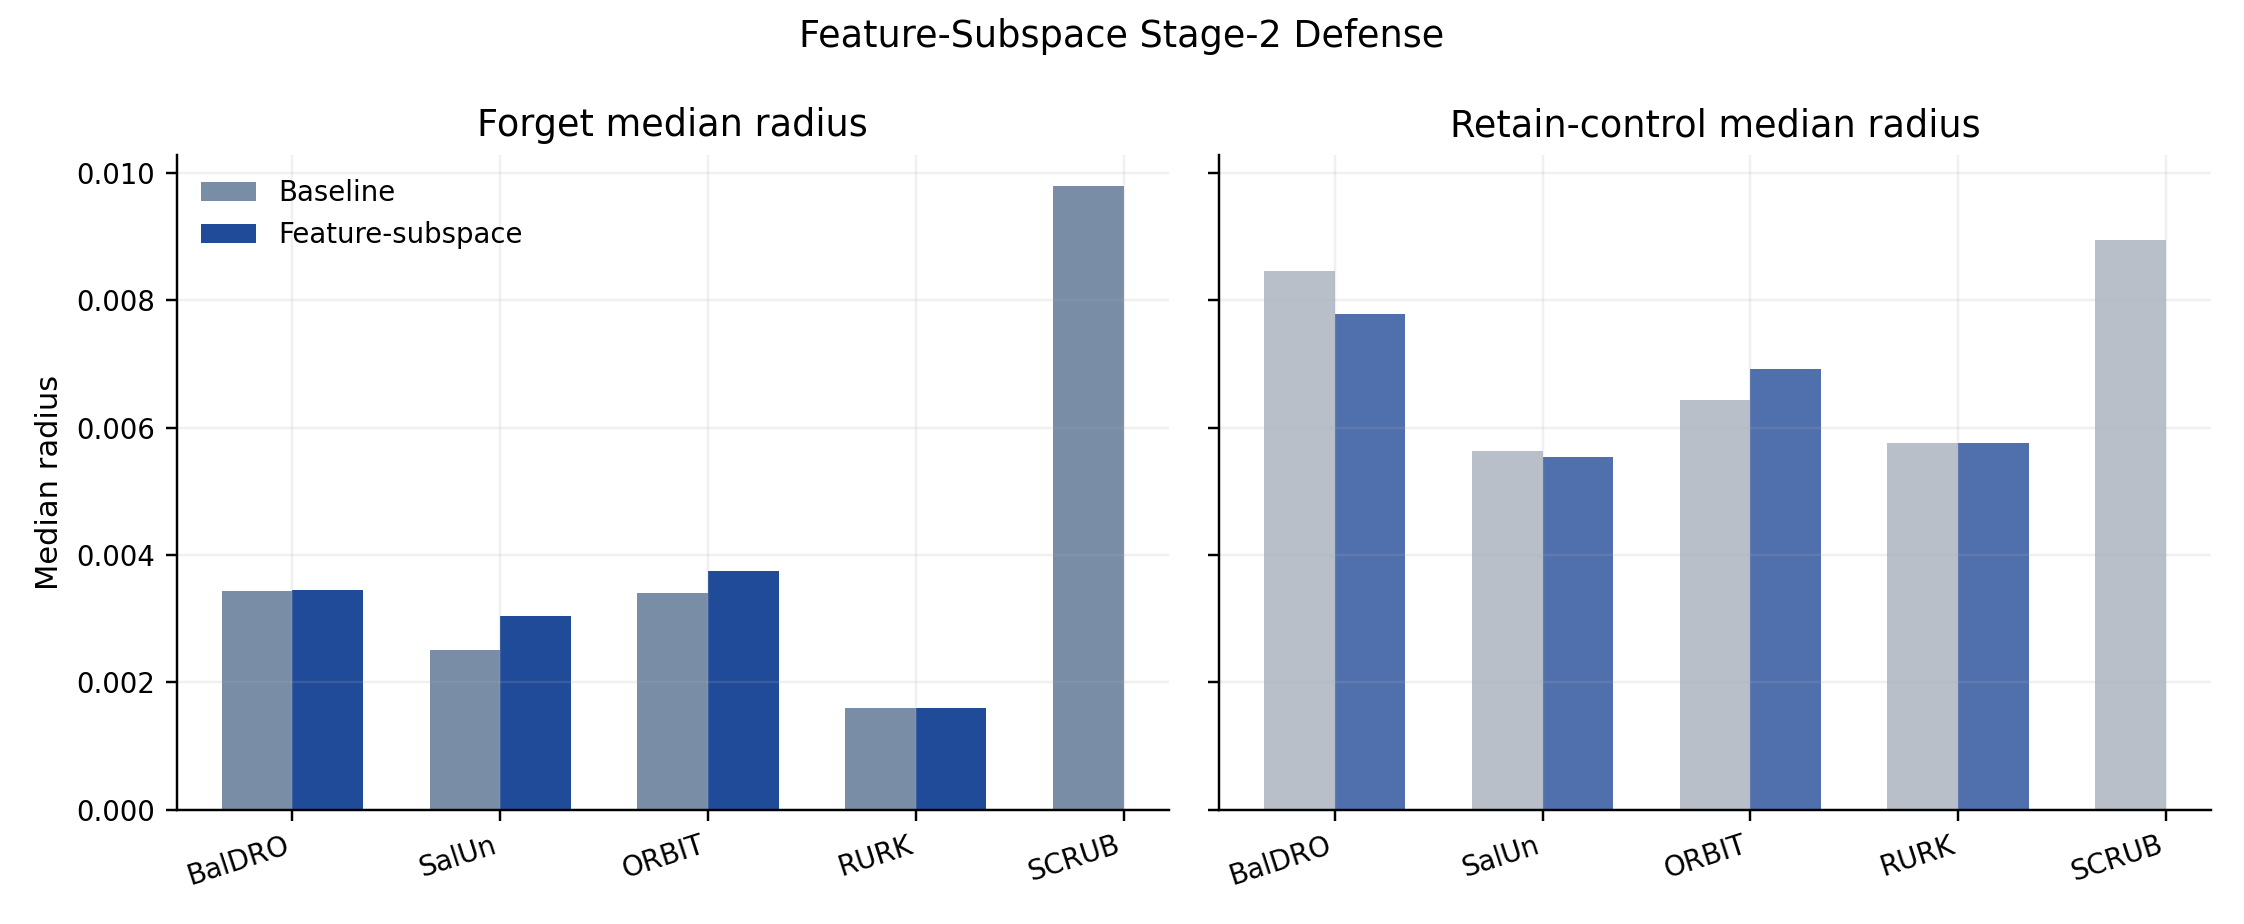
\includegraphics[width=0.92\linewidth]{feature_subspace_tradeoff.png}
  \caption{Feature-subspace stage-2 tradeoff. Larger forget medians indicate stronger resistance to conditional recovery. The plotted point estimates improve most clearly on ORBIT and SalUn, shift only slightly on BalDRO, and do not move RURK. Controlled paired confidence intervals require re-auditing matched-attack baselines from reproducible checkpoints and remain future work.}
\label{fig:subspace-tradeoff}
\end{figure}

\paragraph{Feature-subspace stage-2 defense.}
The most promising post-hoc defense family in the current benchmark is a feature-subspace stage-2 finetune. Rather than modifying the entire forgetting objective from epoch 0, the defense begins from an already-unlearned adapter and suppresses attacked forget-sample features inside a learned recovery subspace. This regime avoids the instability of earlier logit-margin defenses and produces positive point-estimate shifts on BalDRO, SalUn, and ORBIT. The effect is clearest on ORBIT and SalUn; the BalDRO shift is numerically tiny, and the table does not yet include the paired confidence intervals needed to treat it as statistically established. The effect is modest in absolute magnitude because the benchmark is CIFAR-10 under an $L_\infty$ budget on 224$\times$224 inputs, where successful radii are numerically small by construction. What matters in the current evidence is that some rows shift the forget-vs-retain frontier in the right direction without sacrificing clean retain utility, not that feature-subspace training is a universal defense.

\paragraph{CE-U as a core baseline.}
CE-U belongs in the main benchmark even though its first qualified positive defense row appears in the patch regime rather than under full-image recovery. Under the 2-step pilot audit (n=8, seed 42), the baseline CE-U checkpoint has forget median 0.00368 with 0\% clean forget success, and retain-control attacks succeed 0 of 8 times within the $\epsilon$ budget. This is suggestive pilot evidence for selectivity, but it is not ranked against SalUn or ORBIT because those rows use larger full audits. CE-U full-image feature-subspace stage-2 variants are at best flat, and the combined row is slightly worse under the APGD cross-check, so the CE-U defense claim is reserved for the qualified combined stage-2 patch result discussed below.

\begin{figure}[t]
  \centering
  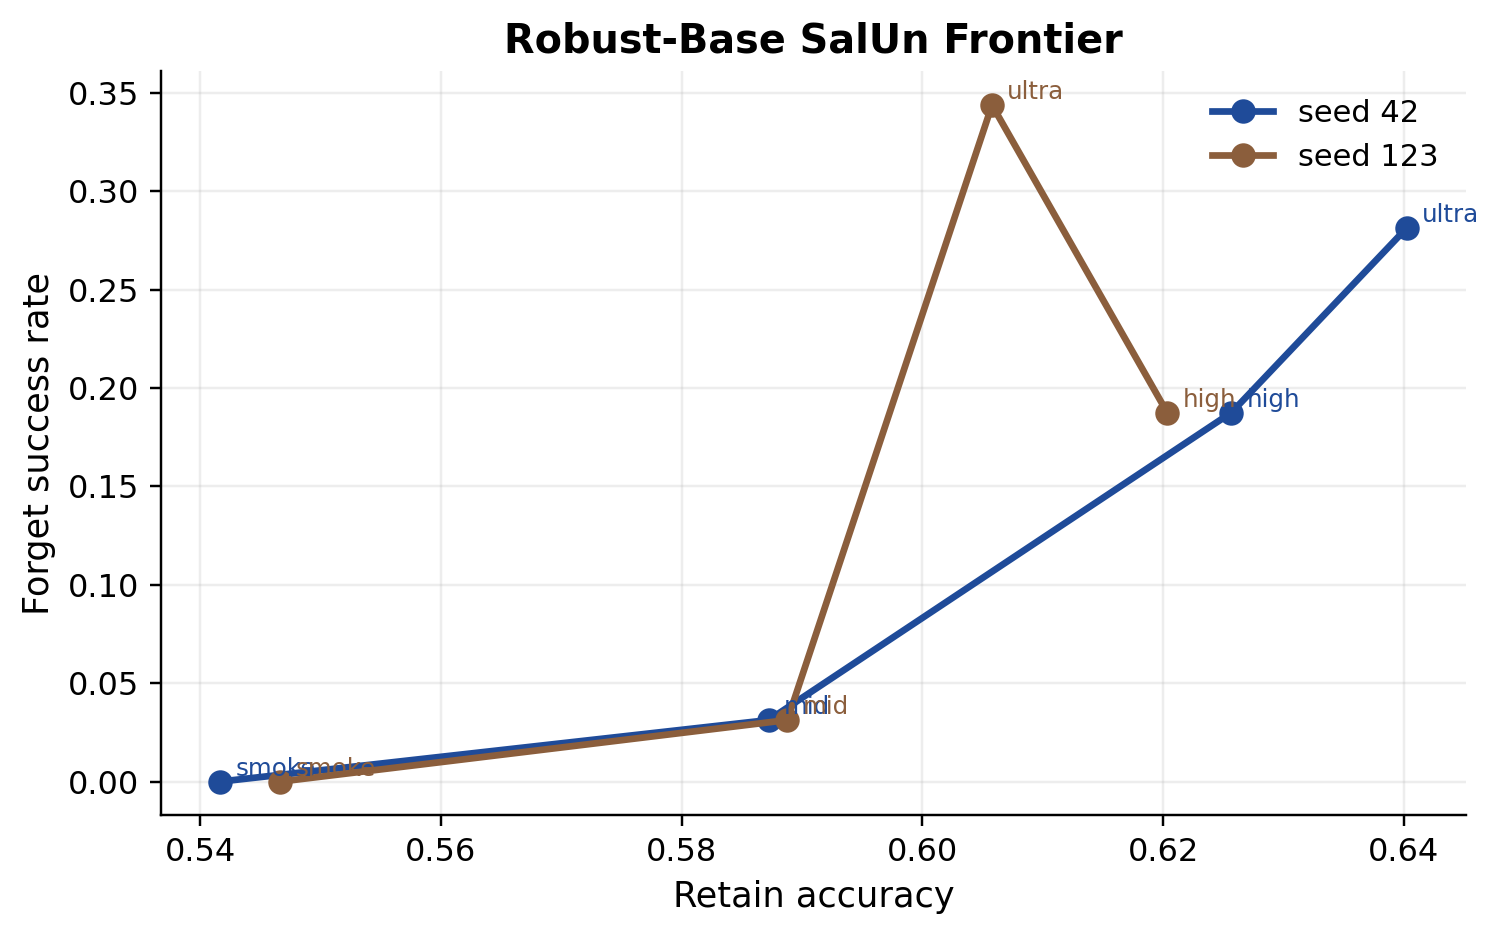
\includegraphics[width=0.92\linewidth]{robust_base_frontier.png}
  \caption{Robust-base SalUn frontier. Lower-utility robust-base checkpoints suppress conditional recovery more strongly, but leakage returns as retain utility improves.}
  \label{fig:robust-frontier}
\end{figure}

\paragraph{Robust-base frontier.}
Robust-base SalUn does not behave like a binary defense success. Instead, it exposes a frontier: at low utility, conditional recovery can drop to zero on the sampled audit; as retain accuracy rises, recovery reappears. This is a stronger framing than a single checkpoint claim because it shows that robustness and post-unlearning utility are coupled. Robust-base training is therefore treated as an operating-point choice rather than a one-shot fix.

\begin{figure}[t]
  \centering
  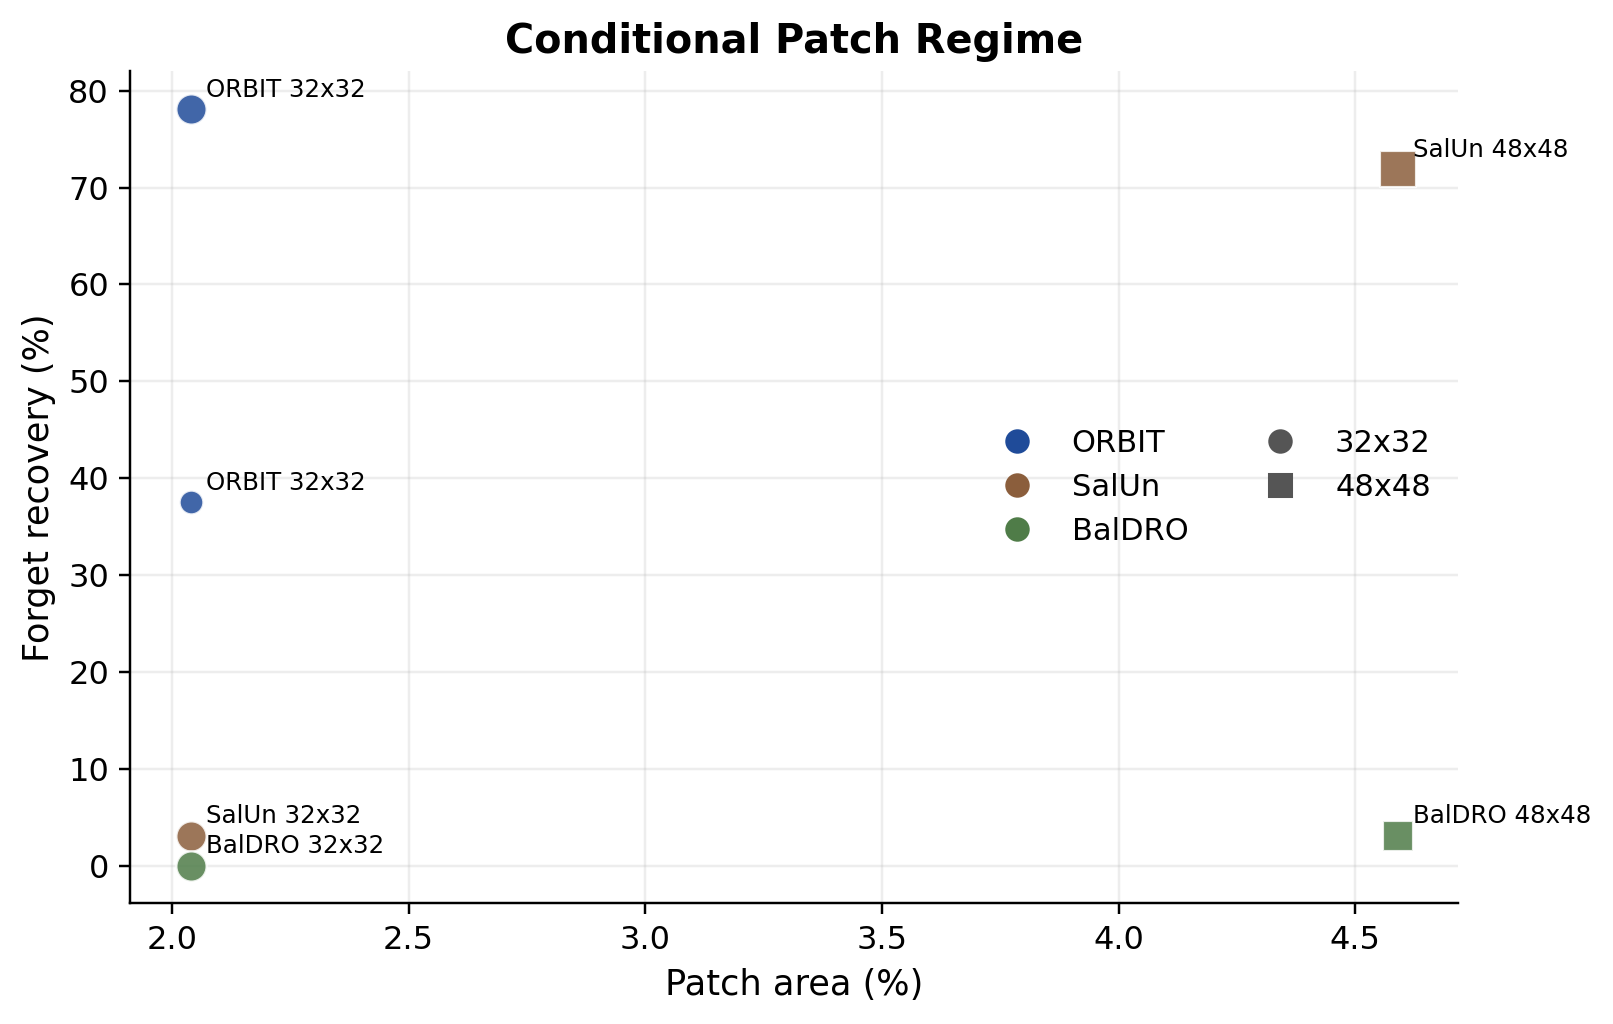
\includegraphics[width=0.92\linewidth]{conditional_patch_regime.png}
  \caption{Conditional patch regime. ORBIT admits strong low-area patch recovery, SalUn requires a larger patch and incurs more retain damage, and BalDRO is effectively negative under the same patch family.}
  \label{fig:patch-regime}
\end{figure}

\paragraph{Conditional patches.}
The patch result is not a universal trigger. Universal static patches were mostly ineffective on the stronger methods. The viable regime is instead a conditional small-area patch attack whose content and placement depend on the input. ORBIT is the flagship positive case: a 32$\times$32 patch covering 2.04\% of the image recovers forgotten behavior strongly while inducing no retain-to-forget hijack. SalUn is patch-vulnerable only at a larger 48$\times$48 budget, and BalDRO is effectively negative at both tested patch sizes. This method dependence reinforces the broader paper thesis: residual forgetting leakage is structured, but not universal.

\paragraph{Delivery surfaces beyond one patch.}
The later delivery-surface checks strengthen the attack story and narrow the defense story. Conditional frame attacks and conditional multi-patch attacks are both real local delivery surfaces, but they do not behave like simple extensions of the one-patch regime. Patch-aware defenses that help on one square patch often fail to transfer: the ORBIT patch-stage2 row becomes easier to recover under the frame attack, CE-U combined stage-2 also becomes easier and adds retain-side failure under the frame attack, and faithful full-ft SalUn patch-stage2 becomes easier under multi-patch delivery. The main exception is weak positive transfer from the ORBIT patch-stage2 row to multi-patch delivery. Frame and multi-patch regimes are therefore treated as first-class red-team surfaces rather than appendix-only perturbation variants.

\paragraph{Second-wave defenses.}
Two later branches sharpen the story. First, teacher-guided stochastic CVaR provides a small but reproducible full-image defense improvement on ORBIT across two seeds, whereas the same probabilistic family remains neutral on CE-U. Second, a combined subspace-plus-patch stage-2 defense gives the first CE-U row that improves under matched Adam audits while also reducing conditional patch success, although its APGD result is still slightly worse than baseline. By contrast, the larger mixed-surface stage-2 defense was explicitly designed to transfer across one-patch, frame, and multi-patch delivery and failed to do so reliably. These later rows are therefore useful but qualified: they extend the defense story beyond pure feature-subspace training without becoming universal fixes.

\paragraph{Takeaway.}
The combined evidence supports a multi-regime view of red-teaming machine unlearning. Strong per-example conditional attacks remain the main threat, conditional patches expose an additional local attack surface on some methods, and frame plus multi-patch attacks show that local-delivery robustness is materially harder than one-patch robustness alone. The best defense families found here are modest and method-specific: feature-subspace stage-2 gives the clearest point-estimate gains on ORBIT and SalUn, teacher-guided stochastic CVaR helps ORBIT slightly, and CE-U combined stage-2 is only a qualified partial row. RURK remains a hard case, and SCRUB serves as a seed-sensitive negative control where generic adversarial fragility usually overwhelms forget-specific interpretation.


\section{Short-Budget and Auxiliary Regimes}
\subsection{Amortized short-budget attack}
The learned distilled short-budget attacker is a real but target-dependent contribution. It improves matched low-step Adam on the repo-defined ORBIT row across both seeds and also helps on SalUn, but it does not preserve a clean forget/retain Pareto on RURK. I therefore position it as an amortized attack regime rather than a universal attack method.

\begin{table}[t]
  \centering
  \small
  \begin{tabular}{l l c c c c}
    \toprule
    Target & Seed & Attack & Forget Succ. & Retain Succ. & Forget Median \\
    \midrule
    ORBIT & 42 & 2-step Adam & 9.4\% & 0.0\% & 0.02500 \\
    ORBIT & 42 & Distilled + 2-step refine & 18.8\% & 0.0\% & 0.02083 \\
    ORBIT & 123 & 2-step Adam & 18.8\% & 0.0\% & 0.00316 \\
    ORBIT & 123 & Distilled + 2-step refine & 31.2\% & 3.1\% & 0.01189 \\
    SalUn & 42 & 2-step Adam & 71.9\% & 9.4\% & 0.00435 \\
    SalUn & 42 & Distilled + 2-step refine & 84.4\% & 9.4\% & 0.00447 \\
    SalUn & 123 & 2-step Adam & 68.8\% & 6.2\% & 0.00328 \\
    SalUn & 123 & Calibrated distilled + 2-step refine & 81.2\% & 12.5\% & 0.00389 \\
    RURK & 42 & 2-step Adam & 87.5\% & 6.2\% & 0.00175 \\
    RURK & 42 & Calibrated distilled + 2-step refine & 90.6\% & 18.8\% & 0.00175 \\
    \bottomrule
  \end{tabular}
  \caption{Short-budget comparison between matched 2-step Adam and the learned distilled conditional attacker. The learned attacker helps most on ORBIT, helps on SalUn with a weaker forget/retain Pareto, and does not remain selective on RURK.}
  \label{tab:short-budget}
\end{table}


\subsection{Earlier prompt/probe regime}
An earlier prompt-style red-team branch found a strong effect on Uniform KL under an oracle-contrastive probe, but not on the stronger methods. In particular, the strongest earlier prompt result moved Uniform KL seed 42 from 12.70\% forget to 21.10\% forget with only a 0.36pp retain drop, while SalUn, SCRUB, and the repo-defined ORBIT row remained in the resistant bucket under that family. I treat this as supporting evidence for regime sensitivity rather than as the core attack result.

\subsection{Uniform KL as a bridge target}
Uniform KL also remains useful under the newer conditional-recovery regime. A fast matched pilot with 2-step \texttt{adam\_margin} on seed 42 recovers all sampled forget examples with median radius 0.00147 while succeeding on only one of eight sampled retain controls. The same pilot on seed 123 is completely flat. This makes Uniform KL a bridge target between the older probe story and the newer conditional-optimization story: it is not only probe-vulnerable, but also locally recoverable on the vulnerable seed. A conditional 32$\times$32 patch on seed 42 also yields a weak but nontrivial patch result (15.6\% forget recovery and 0\% retain-to-forget success), which is enough to show that KL is patch-accessible without making it a flagship patch case.

\subsection{Additional auxiliary targets}
SGA is another useful auxiliary target from the recent related-work list, but the full conditional audit does not support a selective-leakage reading. Across seeds 42, 123, and 456, forget and retain-control success rates are both near ceiling, so this row looks like generic adversarial fragility rather than a meaningful forget-vs-retain gap. A matched 32$\times$32 conditional patch is negative on seed 42, and a lightweight feature-subspace stage-2 pilot yields only marginal improvement. I therefore treat both Uniform KL and SGA as auxiliary regime-defining targets rather than as the main methods around which to build the defense story.

\begin{table}[t]
  \centering
  \small
  \resizebox{\linewidth}{!}{%
  \begin{tabular}{l l l c c c}
    \toprule
    Target & Seed & Regime & Forget Succ. & Retain Succ. & Forget Median / Alpha \\
    \midrule
    Uniform KL & 42 & 2-step conditional pilot & 100.0\% & 12.5\% & 0.00147 \\
    Uniform KL & 123 & 2-step conditional pilot & 0.0\% & 0.0\% & N/A \\
    Uniform KL & 42 & 32x32 conditional patch & 15.6\% & 0.0\% & 0.15234 \\
    Uniform KL & 42 & feature-subspace stage-2 pilot & 100.0\% & 12.5\% & 0.00147 \\
    SGA & 42 & full conditional audit & 100.0\% & 100.0\% & 0.00294 \\
    SGA & 123 & full conditional audit & 96.9\% & 100.0\% & 0.00968 \\
    SGA & 456 & full conditional audit & 96.9\% & 96.9\% & 0.01091 \\
    SGA & 42 & 32x32 conditional patch & 0.0\% & 0.0\% & N/A \\
    SGA & 42 & 2-step baseline pilot & 75.0\% & 0.0\% & 0.00417 \\
    SGA & 42 & 2-step stage-2 pilot & 62.5\% & 0.0\% & 0.00441 \\
    \bottomrule
  \end{tabular}
  }
  \caption{Auxiliary seed-sensitive targets. Uniform KL is a bridge case between the older probe regime and the newer conditional-recovery regime, while SGA is conditional but not patch-local and only shows a weak positive defense pilot on its selective seed.}
  \label{tab:aux-targets}
\end{table}


\section{Empirical Validation of the Theory}
\label{sec:validation}
Each of the four theorems in Section~\ref{sec:theory} comes with a benchmark check. This section reports those checks; together they re-cast the regimes above as theorem tests rather than standalone attack curves.

\subsection{Theorem~\ref{thm:gap}: the recovery--certification scatter}
For each method I estimate the margin-Jacobian Lipschitz proxy $\hat L$ from the Jacobian-access audit and the median recovery radius $\mathrm{median}(\hat r)$ from the recovery-radius audit, joining $40$ (method, seed, config) rows. Figure~\ref{fig:lip-scatter} plots them against the bound $\hat r \geq -\bar m/\hat L$ of Eq.~\eqref{eq:thm1-pointwise}. The proxies separate the methods cleanly: $\hat L \approx 47$ for SCRUB, $26$ for ORBIT, $16$ for Uniform-KL, and $15$ for SalUn. Inverting Corollary~\ref{cor:cert} at $\gamma = 2$, $B = 10$ gives the \emph{floor} on each method's honest certificate $\epsilon_c$---the tightest budget the audit does not already falsify: SCRUB $0.013$, ORBIT $0.034$, SalUn $0.048$, Uniform-KL $0.050$. The most easily recovered method (Uniform-KL, smallest median radius) is forced to the largest floor, i.e.\ the weakest honest certificate, exactly as the bound predicts. SCRUB's Lipschitz constant is about $3\times$ ORBIT's and SalUn's, and this is the same fact that makes its selective gap vanish under Theorem~\ref{thm:pinsker}: a large $\hat L$ lets small perturbations swing the margin both selectively and non-selectively, so the method looks generically fragile rather than selectively leaky.

\begin{figure}[t]
  \centering
  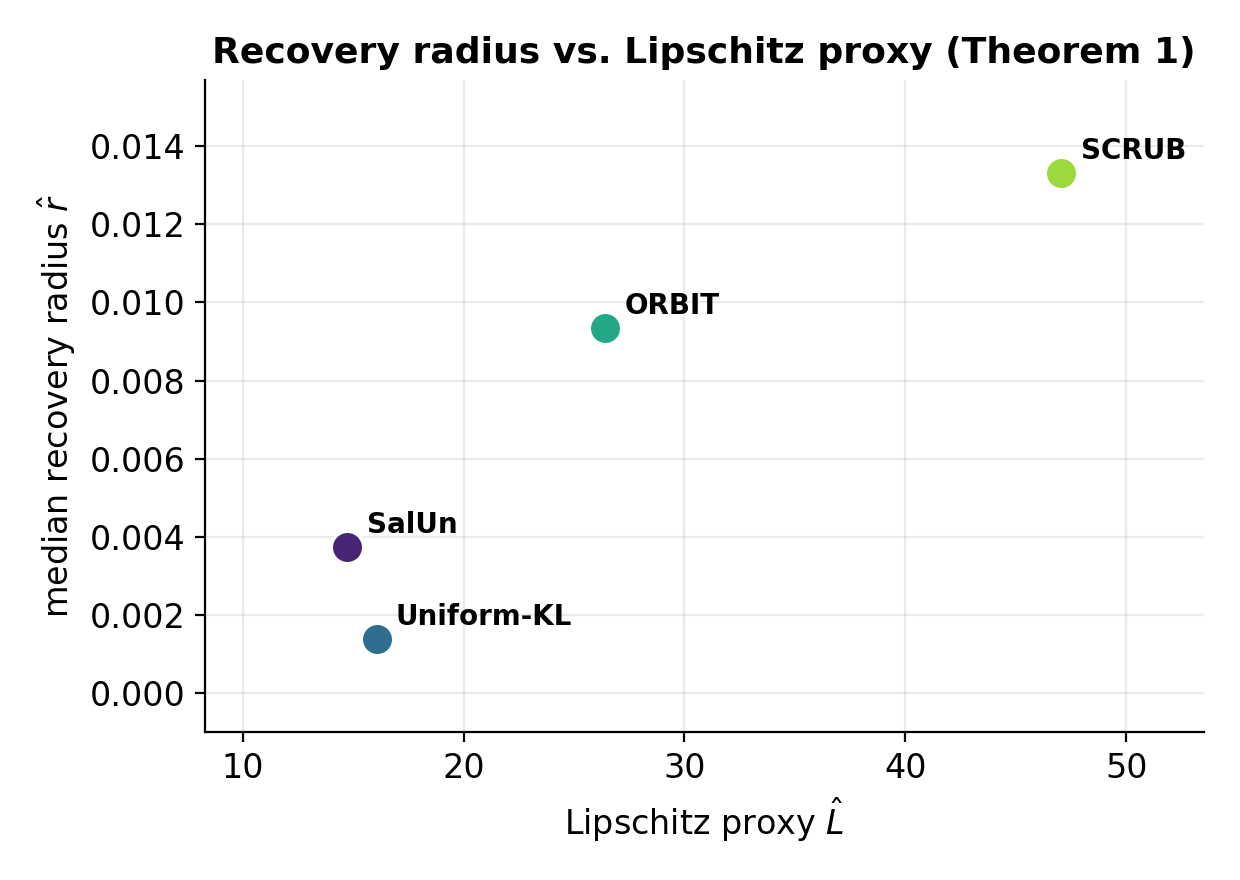
\includegraphics[width=0.92\linewidth]{lipschitz_radius_scatter.png}
  \caption{Theorem~\ref{thm:gap} check. Per-method Lipschitz proxy $\hat L$ versus median recovery radius $\hat r$, one point per (method, seed). Methods on the bound line $\hat r = -\bar m/\hat L$ are tight; methods above it have margin headroom. SCRUB's large $\hat L$ lets small perturbations swing the margin, which explains its near-zero selective gap under Theorem~\ref{thm:pinsker}.}
  \label{fig:lip-scatter}
\end{figure}

\subsection{Theorem~\ref{thm:pinsker}: the Pinsker KL table}
I compute the forget and retain-control recovery rates $(\hat p_F, \hat p_R)$ for $226$ (method, seed, audit-config) rows and report the Pinsker lower bound $\mathrm{KL} \geq 2|\hat p_F - \hat p_R|^2$ (and the tighter Bretagnolle--Huber bound) in \texttt{results/analysis/reports/pinsker\_kl\_table.md}. The ordering is the one the qualitative story predicted, now with a quantitative gap. CE-U recovers $\hat p_F = 0.875$ of forget examples against $\hat p_R = 0.000$ retain controls ($|\Delta| = 0.875$); SalUn sits near $|\Delta| \approx 0.625$; ORBIT shows a positive but smaller selective gap. SCRUB sits at the bottom with $\hat p_F \approx \hat p_R \approx 0.97$ and $|\Delta| \approx 0.031$, forcing a KL lower bound of only $\approx 0.002$. By Corollary~\ref{cor:scrub} this formally certifies SCRUB as a \emph{vacuous} selective-leakage case at the audited scale: its strong attack success carries essentially no information about the forget condition, so it is generic adversarial fragility, not unlearning failure.

\subsection{Theorem~\ref{thm:transfer}: covering implies the mixed-surface failure}
The patch, border-frame, and multi-patch results reported above are the empirical witness for Theorem~\ref{thm:transfer}. Patch-aware stage-2 closes the single-patch channel on ORBIT and CE-U, but the same defense becomes easier to recover under frame and multi-patch delivery, and mixed-surface stage-2---explicitly trained on multiple surfaces---does not reliably fix the transfer gap. Under Lemma~\ref{lem:cover}, the union of $32\times 32$ patches and $16$-pixel frames is covering, so worst-case robustness across the family is equivalent to input-invariance and forces constancy (Corollary~\ref{cor:no-free-lunch}). The mixed-surface failure is therefore not an engineering artifact but the only possible outcome for a non-trivial classifier; the constructive consequence is to retarget local-delivery defense at realistic (non-covering) stochastic delivery priors rather than worst-case invariance.

\subsection{Theorem~\ref{thm:smooth}: predicted vs.\ measured certified radius}
The smoothed objective of Eq.~\eqref{eq:smoothed} is implemented as \texttt{SmoothedMarginUnlearning} and trained end-to-end on seed 42. Starting from a base ViT-Tiny at $94.2\%$ validation accuracy, a 10-epoch smoothed-margin LoRA fine-tune ($\sigma = 0.10$, $n_{\text{noise}} = 4$, $\gamma = 1.0$) drives forget accuracy $95.7\% \to 12.0\%$ while retain accuracy is preserved ($93.9\% \to 93.8\%$). The smoothed certified-radius audit ($n_{\text{noise}} = 256$, $\alpha = 10^{-3}$, 64 forget + 64 retain) certifies a median $L_2$ radius $R = 0.193$ from Theorem~\ref{thm:smooth}. The matched recovery audit gives forget median $\epsilon = 0.00176$ against retain median $\epsilon = 0.00613$---a $3.5\times$ selective gap. Here the selectivity is carried by the recovery \emph{radius} (the Theorem~\ref{thm:gap} object) rather than the binary recovery rate of the Pinsker test: both splits saturate near $\hat p_F \approx \hat p_R \approx 1$ at $\epsilon_{\max}$, so the radius separation, not the rate gap, is the informative signal at this budget. Figure~\ref{fig:pred-meas} joins $128$ samples: there are zero retain-side certificate violations, and the ten forget-side ``violations'' are all clean-leak cases where the un-smoothed model already predicts the forgotten class on the clean input while the smoothed classifier remains robust---a positive signal for smoothing, not a counterexample to the certificate.

\begin{figure}[t]
  \centering
  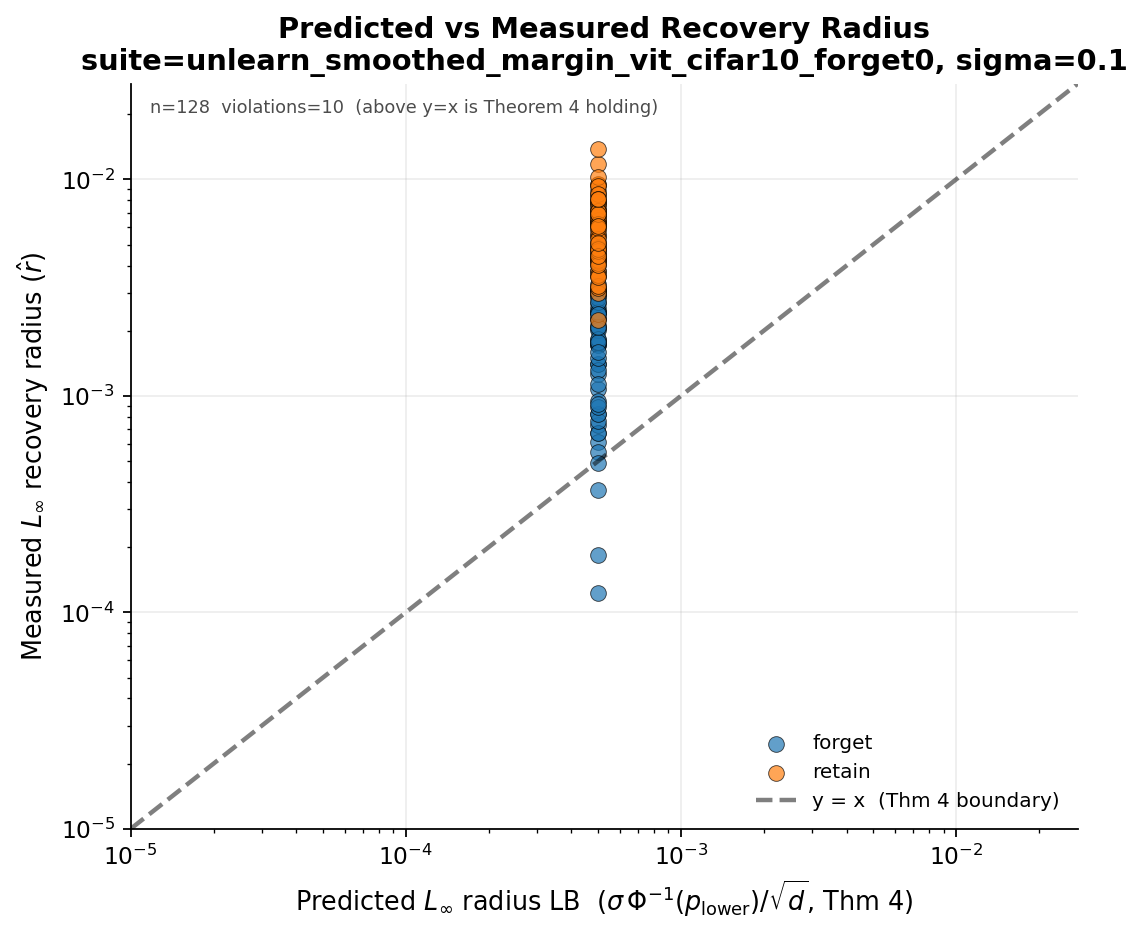
\includegraphics[width=0.92\linewidth]{predicted_vs_measured_radius.png}
  \caption{Theorem~\ref{thm:smooth} check. Predicted Cohen--Rosenfeld--Kolter certified radius versus measured recovery radius for the smoothed-margin unlearner (seed 42). Zero retain-side violations; the forget-side points below the line are clean-leak cases on the \emph{un}-smoothed model, which the smoothed classifier corrects.}
  \label{fig:pred-meas}
\end{figure}

\section{Defense Discussion}
\subsection{Feature-subspace stage-2}
The first defense family that consistently helps is a post-unlearning feature-subspace stage-2 finetune. Instead of modifying the full unlearning objective from epoch 0, I begin from an already-unlearned adapter and suppress attacked forget-sample features inside a learned recovery subspace. This avoids the instability of earlier logit-margin and teacher-distillation defenses on BalDRO.

\subsection{Why the gains are small}
The absolute changes in reported radii are numerically small because the benchmark itself is small: CIFAR-10 under an $L_\infty$ budget on 224$\times$224 inputs yields radii on the order of a few thousandths. The right question is therefore relative: does the defense move the forget-vs-retain frontier without collapsing clean utility? On BalDRO, SalUn, and the repo-defined ORBIT row, the answer is yes, though modestly.

\subsection{What does not generalize}
The defense is not universal. RURK remains a hard case under both attack and defense. SCRUB behaves like generic adversarial fragility rather than a clean forgetting-leak regime, so stronger attacks on SCRUB do not necessarily imply a meaningful unlearning failure mode. The newer delivery-surface results make this sharper: patch-aware defenses often fail to transfer to border-frame or multi-patch delivery, and the mixed-surface stage-2 branch does not reliably fix that.

\section{Proposed Defense Objective}
The experiments suggest that clean-point forgetting is too weak a training target. A more principled direction is targeted-margin adversarial unlearning:
\begin{equation}
\min_{\theta}
\mathbb{E}_{x \in R} L_{\text{retain}}(x;\theta)
 + \lambda_f \mathbb{E}_{x \in F} L_{\text{forget}}(x;\theta)
 + \lambda_m \mathbb{E}_{x \in F} \max\!\left(0,\; m_t(x + \delta^*(x)) + \gamma \right),
\label{eq:proposed}
\end{equation}
where $F$ is the forget set, $R$ is the retain set, $m_t$ is the forgotten-class target margin, $\delta^*(x)$ is an inner-loop or amortized attack, and $\gamma$ is a safety margin. This objective is purely empirical: it minimizes a worst-case inner attack and carries no certificate. Theorem~\ref{thm:smooth} upgrades it by replacing the inner attacker $\delta^*(x)$ with Gaussian smoothing of the margin penalty, Eq.~\eqref{eq:smoothed}, which inherits a Cohen--Rosenfeld--Kolter certified recovery radius and (via Corollary~\ref{cor:gen}) a PAC generalization bound to the forget distribution. The end-to-end result in Section~\ref{sec:validation} (forget $95.7\%\to12.0\%$, retain preserved, certified $L_2$ radius $0.193$) is the realized version of this objective. The implemented feature-subspace stage-2 defense can be viewed as a computationally cheaper, uncertified approximation to the same idea: defend against locally recoverable targeted behavior, not just against clean forget accuracy.

\section{Discussion}
This work began as a multi-regime red-team study, and Section~\ref{sec:validation} turns that benchmark into the empirical validation of the small theory of Section~\ref{sec:theory}: the Lipschitz--radius scatter tests Theorem~\ref{thm:gap}, the Pinsker KL table tests Theorem~\ref{thm:pinsker}, the patch/frame/multi-patch transfer failure instantiates Theorem~\ref{thm:transfer}, and the smoothed-margin run realizes Theorem~\ref{thm:smooth}. Read together, the theory explains \emph{why} the empirical picture is non-universal: recovery radius is lower-bounded by a method-specific Lipschitz constant (so SCRUB's large $\hat L$, which lets perturbations swing the margin freely, is what erases its selective gap), and worst-case multi-surface robustness is provably unattainable for a non-trivial classifier. The evidence does not support a universal ``magic'' attack or defense. Strong per-example conditional recovery is the main general threat; universal perturbations are mostly weak on the stronger checkpoints; conditional patches expose an additional local attack surface on some methods; border-frame and multi-patch delivery show that local-delivery transfer is a separate problem; robust-base methods define a utility-vs-recovery frontier rather than a binary robust point; and feature-subspace stage-2 provides the first modest defense gains on several targets. Later defense branches remain method-specific: teacher-guided stochastic CVaR helps the repo-defined ORBIT row slightly but not CE-U, while patch-aware stage-2 gives the first clearly positive CE-U result in the patch regime (68.8\%$\to$43.8\% at 32$\times$32, seed 42) with no retain-side failure, though it does not help on the full-image conditional attack. Mixed-surface stage-2 is informative precisely because it fails: even explicit delivery-surface-aware training does not reliably generalize across one-patch, frame, and multi-patch attacks. Uniform KL reinforces this framing: seed 42 is vulnerable under both the older prompt/probe family and the newer conditional audit, while seed 123 stays flat under the same fast conditional attack. That multifaceted pattern is scientifically stronger than forcing all methods into one attack or defense family.


\section{Limitations}
I do not claim a universally stronger new optimizer than strong first-order attacks such as \texttt{adam\_margin} or \texttt{apgd\_margin}. The amortized short-budget attack is partial and target-dependent. The defense gains are modest and currently demonstrated on a benchmark that is intentionally controlled rather than broad: mostly CIFAR-10 ViT checkpoints, often with LoRA-based unlearning implementations, plus a smaller number of full-finetune and cross-architecture checks. This makes the benchmark useful for discovering failure modes and transfer gaps, but not yet a direct proxy for most industry deletion settings. Finally, some regimes are better understood as negatives or controls than as headline wins.

The theory carries its own caveats, and I state them rather than hide them. (i) The Lipschitz proxy $\hat L$ of Theorem~\ref{thm:gap} is a margin-Jacobian operator-norm estimate at audit points, not a global certificate; a loose $\hat L$ still yields a \emph{valid} lower bound but an unhelpfully large one, so the scatter is informative only where the estimate is tight. The logit-to-margin conversion in Corollary~\ref{cor:cert} additionally assumes bounded logits, and its constant ($4B$) is not optimized. (ii) Pinsker's inequality in Theorem~\ref{thm:pinsker} is loose; I report the tighter Bretagnolle--Huber bound alongside it, but neither is a hypothesis test with finite-sample coverage at the small per-row audit sizes ($n_F = n_R$ from 4 to 32). (iii) The covering assumption of Theorem~\ref{thm:transfer} bites at budget $\epsilon = 1$, whereas the audits use $\epsilon \ll 1$; the impossibility is therefore a statement about the \emph{limit} of worst-case multi-surface robustness, and the practical reading is to retarget defense at non-covering stochastic delivery priors. (iv) Theorem~\ref{thm:smooth} certifies an $L_2$ radius via randomized smoothing, while the recovery audits are $L_\infty$; the two are related only up to a $\sqrt{d}$ conversion penalty, and the end-to-end smoothed-margin result is a single-seed (seed 42) demonstration rather than a multi-seed study. Each of these is a concrete next step, not a hidden assumption.

\section{Conclusion}
Machine unlearning cannot be evaluated reliably with clean forget accuracy alone. This paper makes the per-example recovery radius the central object and shows it supports a small but operational theory: a Lipschitz recovery--certification gap that bounds any claimable certificate (Theorem~\ref{thm:gap}), a Pinsker test that separates selective leakage from generic fragility (Theorem~\ref{thm:pinsker}), a topological impossibility that explains the mixed-surface transfer failure (Theorem~\ref{thm:transfer}), and a smoothed objective with a certified recovery radius (Theorem~\ref{thm:smooth}). Across the benchmark, the dominant leakage channel is strong per-example conditional recovery, but local patch, frame, and multi-patch attacks expose additional method-specific surfaces that do not reduce to a single universal vulnerability, and the defense picture is similarly non-universal: feature-subspace stage-2 helps several rows, patch-aware training helps ORBIT and CE-U locally, and worst-case transfer across delivery surfaces is provably unattainable. The benchmark is no longer the headline; it is the experimental validation of the theory.

\appendix

\section{Appendix: Seed Variance and Baseline Stability}
The clean baseline regime itself is highly variable across seeds for several unlearning methods, especially on forget accuracy. Figure~\ref{fig:seed-variance} summarizes this instability. This is one reason the paper emphasizes attack-conditioned evaluation rather than clean forget accuracy alone.

\begin{figure}[t]
  \centering
  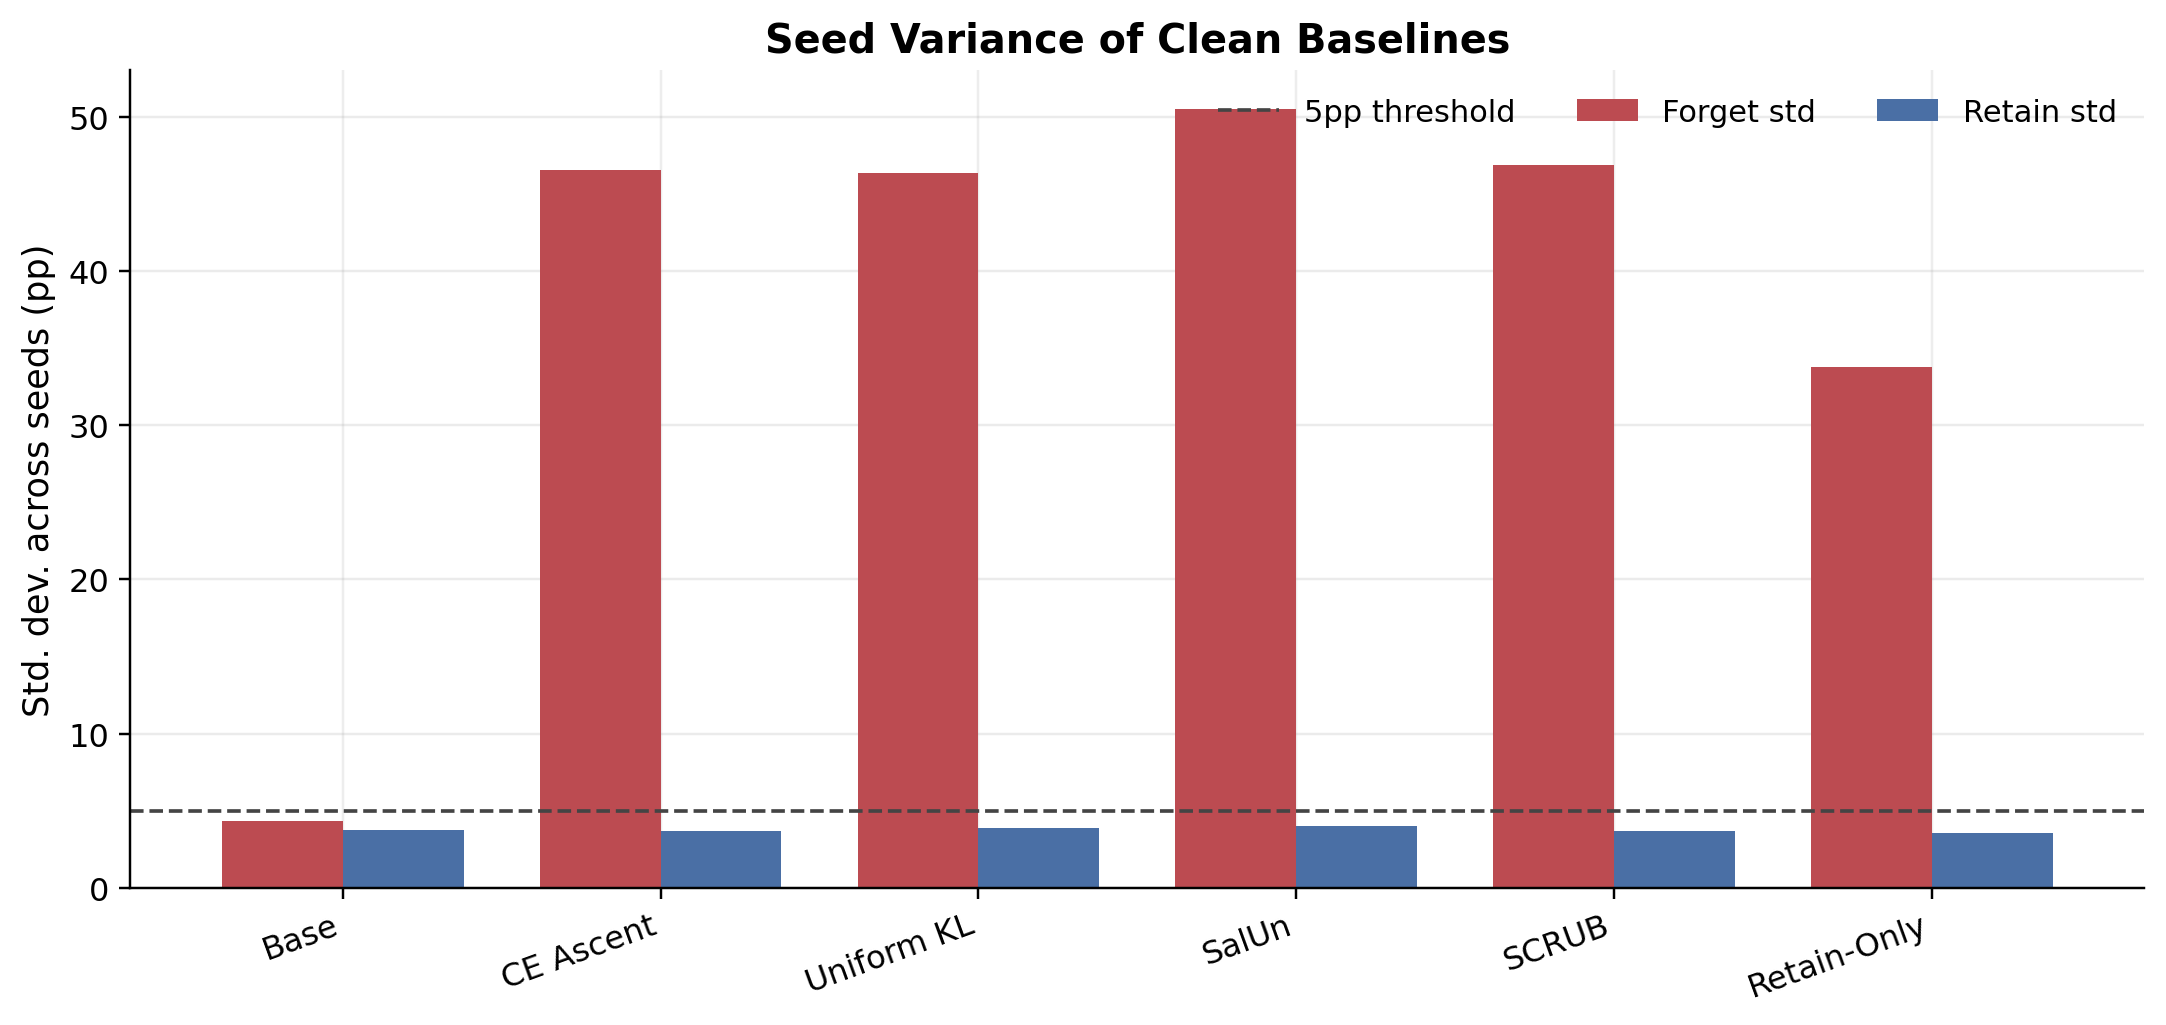
\includegraphics[width=0.92\linewidth]{baseline_seed_variance.png}
  \caption{Seed variance of clean baselines. Forget-side variance is large for several methods even when retain-side variance remains small.}
  \label{fig:seed-variance}
\end{figure}

\section{Appendix: Robust-Base Frontier}
Figure~\ref{fig:robust-frontier} summarizes the robust-base SalUn operating-point story. At low utility, recovery can be suppressed strongly or disappear on the sampled audit. As retain accuracy increases, conditional recovery re-emerges. This makes robust-base training a frontier choice rather than a single robust point.

\begin{figure}[t]
  \centering
  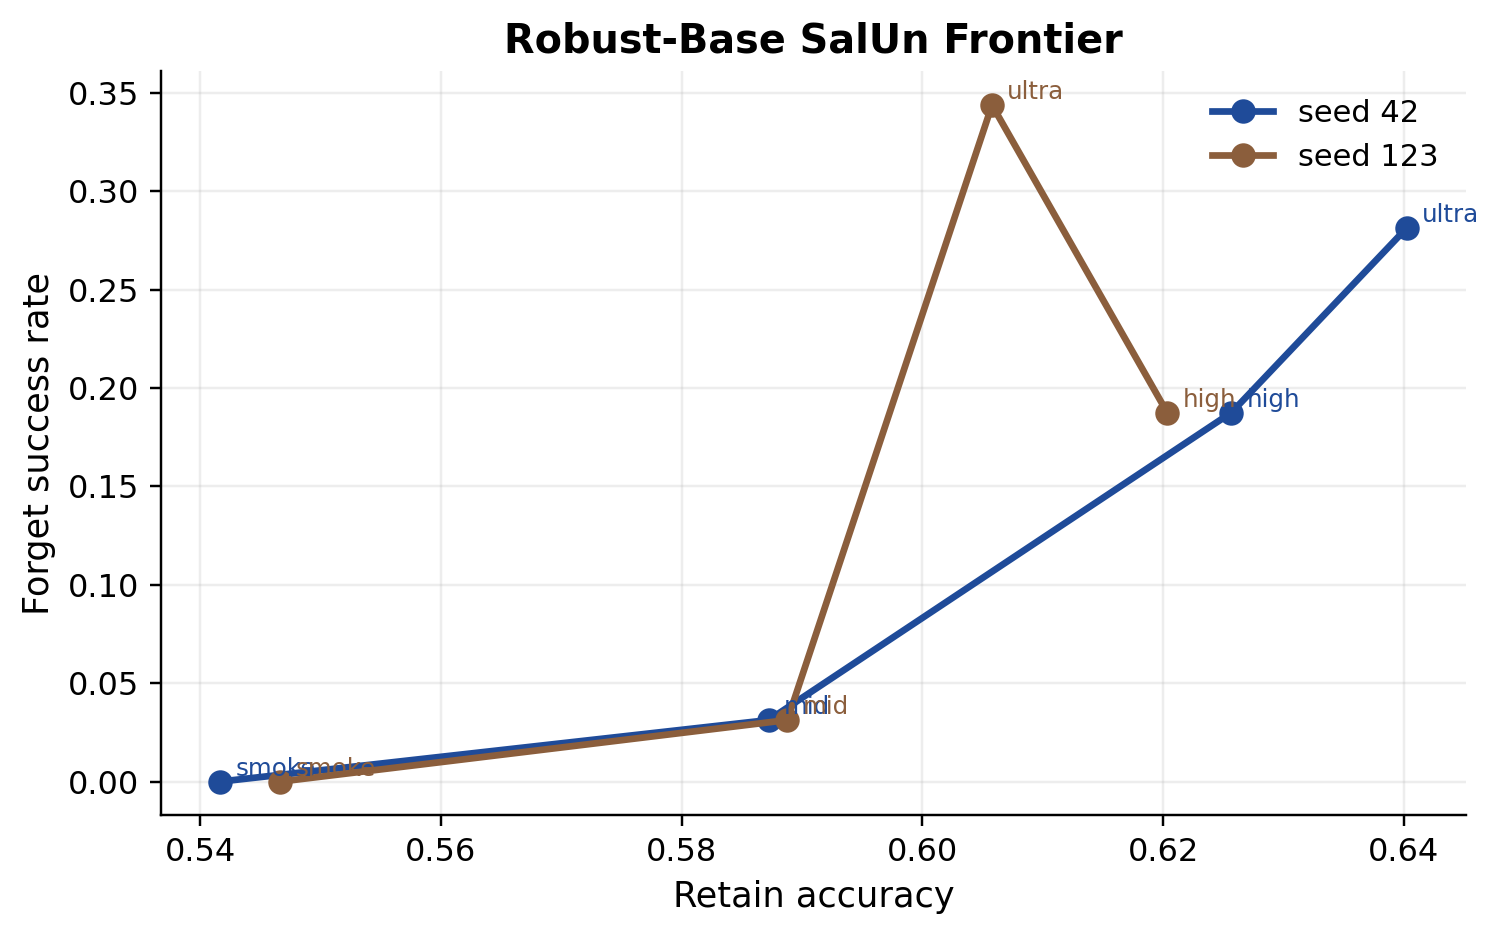
\includegraphics[width=0.92\linewidth]{robust_base_frontier.png}
  \caption{Robust-base SalUn operating-point frontier. Conditional recovery re-emerges as retain accuracy rises, confirming that robust-base training shifts the frontier rather than eliminating leakage.}
  \label{fig:robust-frontier-app}
\end{figure}

\section{Appendix: Conditional Patch Regime}
The patch regime is method-dependent. The repo-defined ORBIT row is the flagship positive case with a 32$\times$32 conditional patch covering 2.04\% of the image, strong forget recovery, 0\% retain-to-forget success, and limited retain accuracy drop. SalUn is patch-vulnerable only at a larger 48$\times$48 patch budget. BalDRO is effectively negative at the tested budgets. Figure~\ref{fig:patch-regime} summarizes the patch success rates across methods and seeds.

\begin{figure}[t]
  \centering
  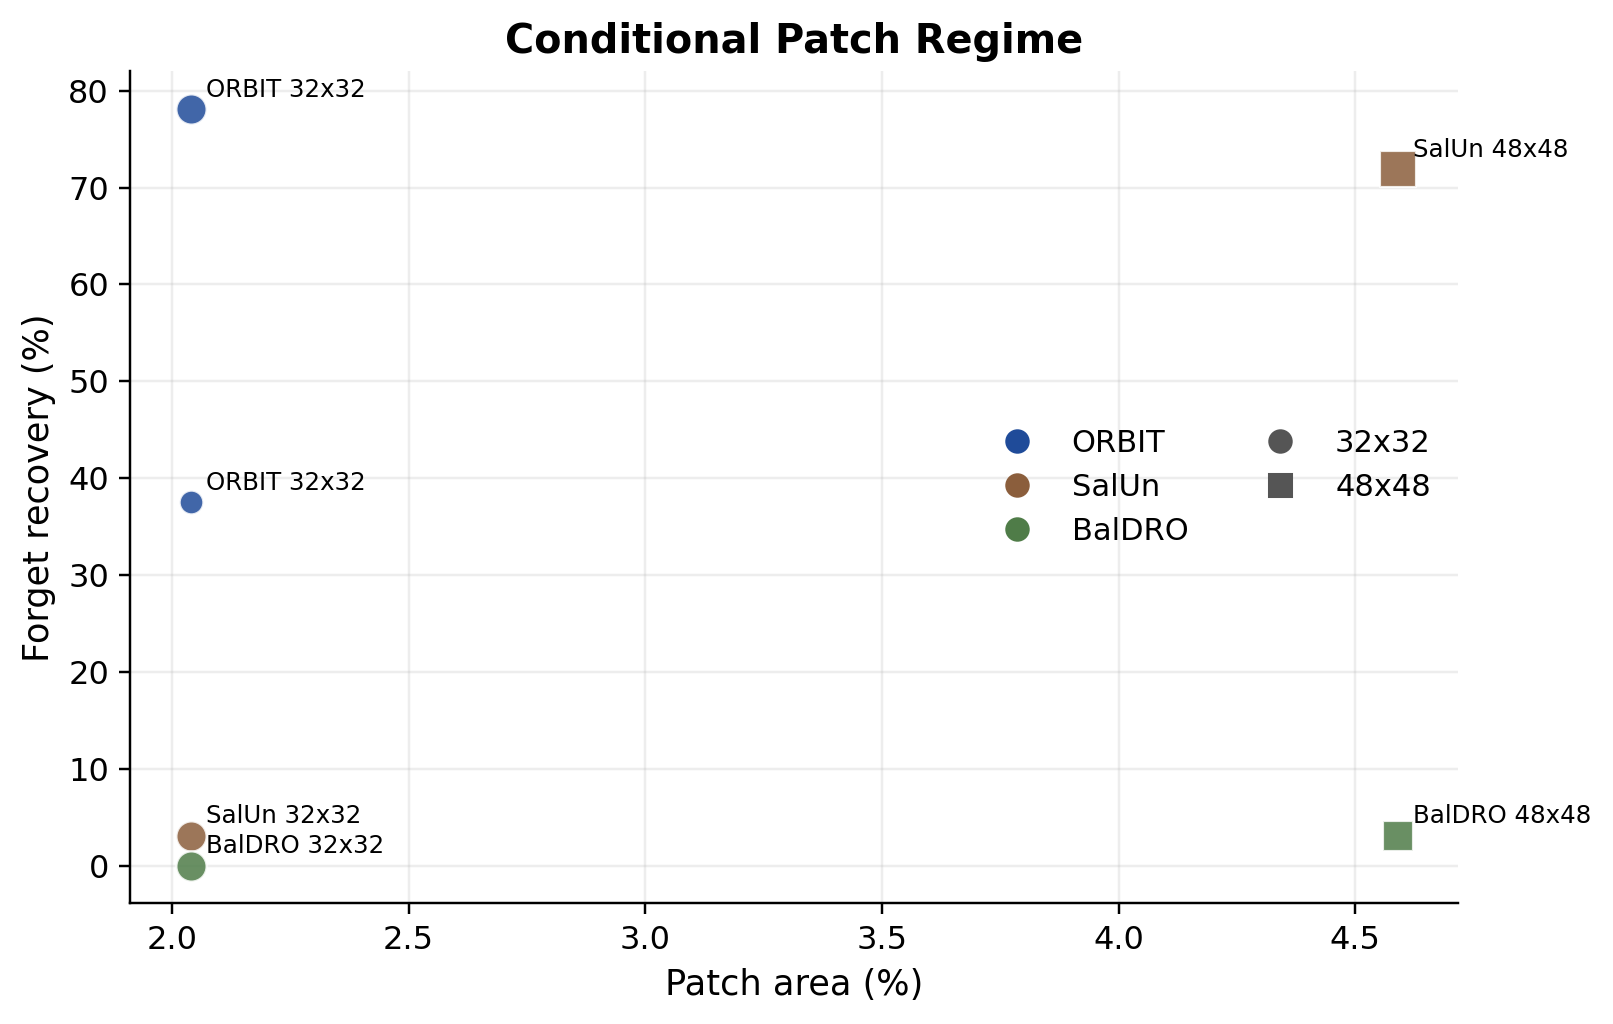
\includegraphics[width=0.92\linewidth]{conditional_patch_regime.png}
  \caption{Conditional patch recovery rates across methods. ORBIT is the strongest patch-positive case; BalDRO and robust-base SalUn are effectively negative at 32$\times$32.}
  \label{fig:patch-regime-app}
\end{figure}

\section{Appendix: Delivery-Surface Transfer}
The later delivery-surface checks separate one-patch wins from broader local-delivery robustness. Under the conditional frame attack, the ORBIT patch-stage2 row and CE-U combined stage-2 both become easier to recover, and CE-U also incurs retain-side failure. Under conditional multi-patch delivery, the ORBIT patch-stage2 row transfers only weakly, while CE-U combined stage-2 and faithful full-ft SalUn patch-stage2 become easier to recover. Mixed-surface stage-2 was designed to fix this transfer problem, but in practice it only gives narrow gains and often worsens frame or multi-patch robustness. I therefore treat delivery-surface transfer as an open defense problem rather than as solved by the current stage-2 families.

\section{Appendix: Negative and Hard Cases}
RURK remains a hard case for both the amortized attack family and the feature-subspace defense. SCRUB is useful as a negative control: strong conditional attacks succeed, but forget and retain-control radii are almost identical, which suggests generic adversarial fragility rather than a clean forgetting-leak mechanism. Several later defense branches also belong in this bucket: mixed-surface stage-2, frame-transfer failures, and the faithful full-ft SalUn mixed-surface row are all informative mainly because they show what does not transfer.

\section{Appendix: Reproducibility Artifacts}
The paper draws from repository summaries and generated figures in:
\begin{itemize}[leftmargin=1.5em]
  \item \texttt{results/analysis/feature\_subspace\_tradeoff.md}
  \item \texttt{results/analysis/recovery\_tradeoff\_summary.md}
  \item \texttt{results/analysis/conditional\_patch\_summary.md}
  \item \texttt{results/analysis/paper\_results\_outline.md}
  \item \texttt{results/analysis/figures/}
\end{itemize}

All figures and tables in this paper are generated from JSON result files committed alongside the code. The repository contains checkpoints for all eight benchmark methods across seeds 42, 123, and 456 together with the audit scripts needed to reproduce each attack regime.

\section{Appendix: Low-Shot Controls}
The lower-shot prompt controls help separate real recovery from trivial prompt memorization. Figure~\ref{fig:kshot-controls} summarizes two useful trends: oracle controls remain flat near zero across the tracked shot counts, while KL and SCRUB can become vulnerable only in specific low-shot or high-shot regimes.

\begin{figure}[t]
  \centering
  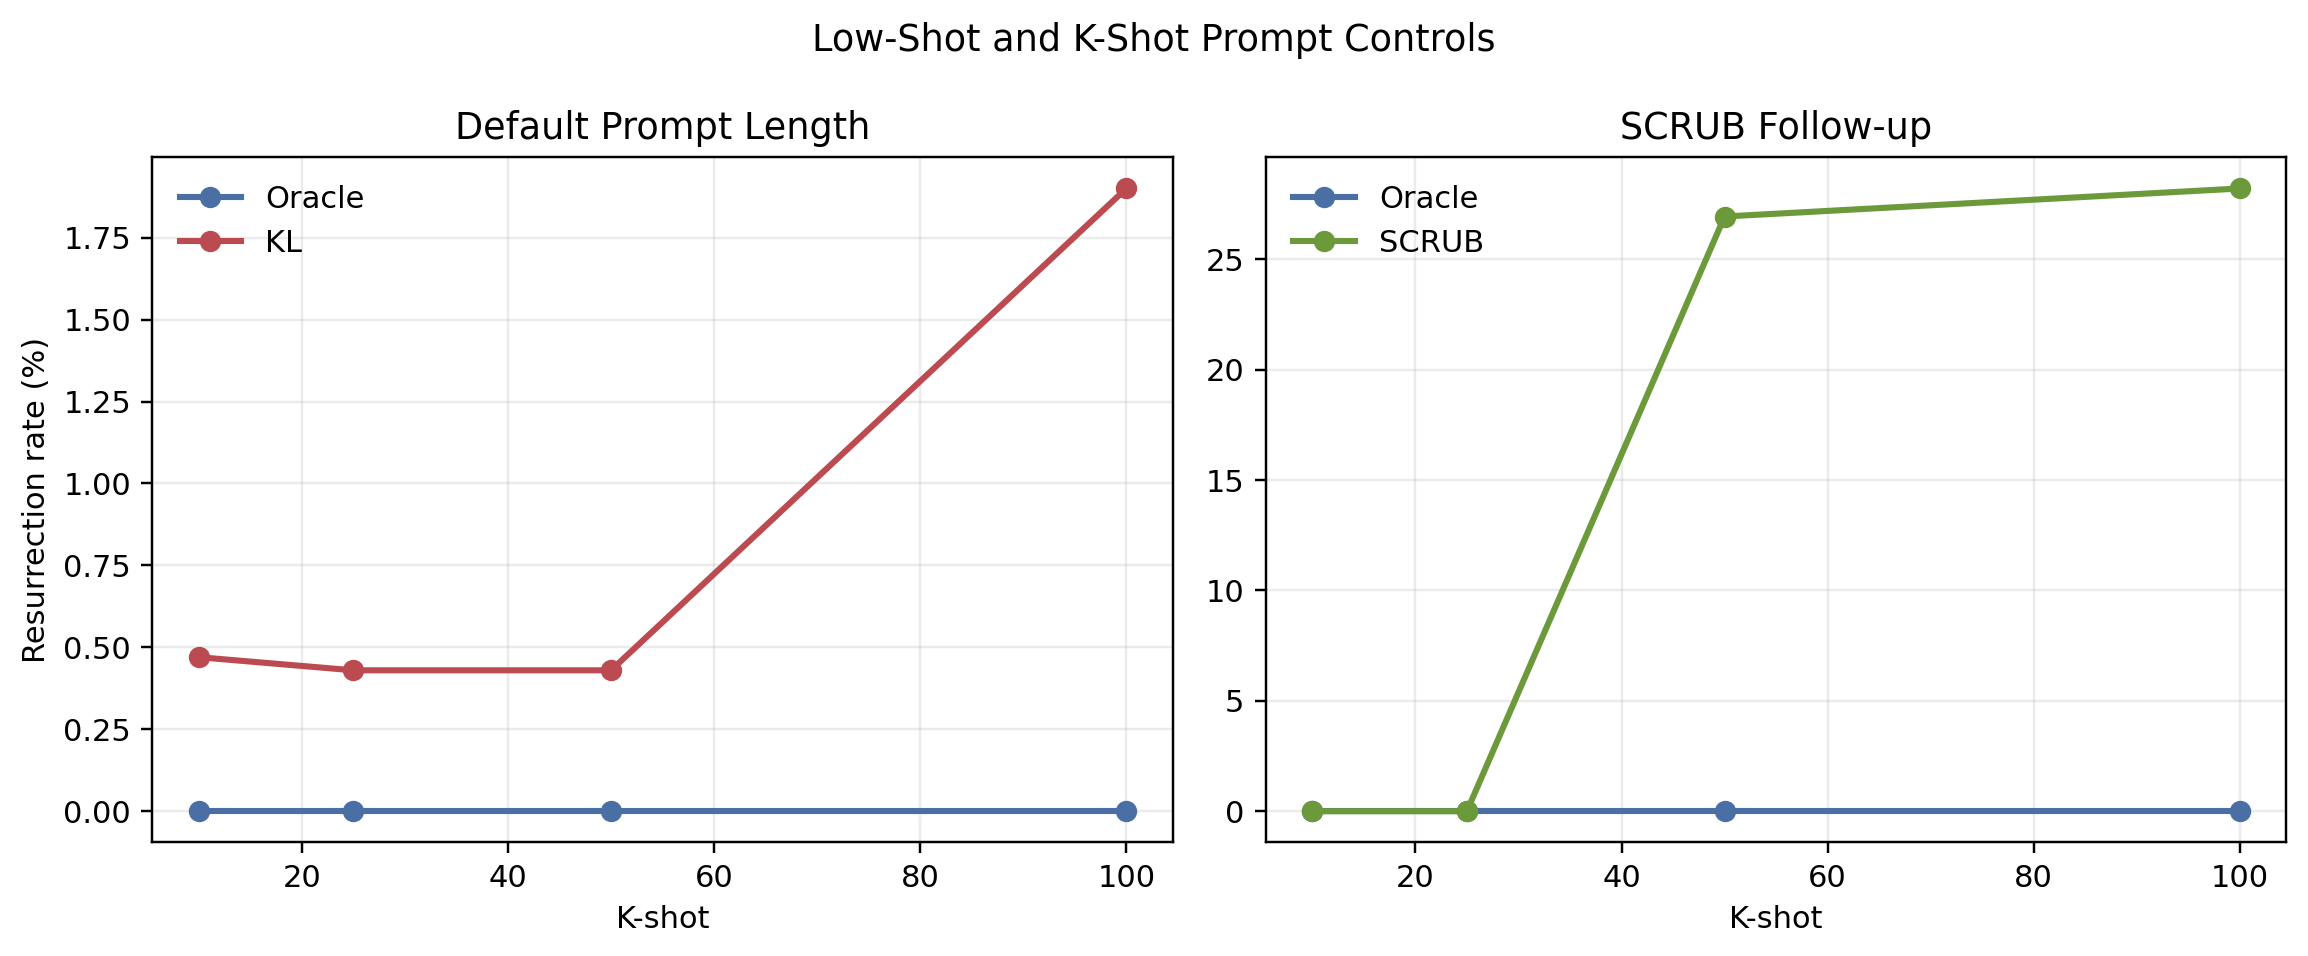
\includegraphics[width=0.92\linewidth]{kshot_controls.png}
  \caption{K-shot prompt controls. Oracle stays flat, KL remains weakly vulnerable, and SCRUB only becomes unstable in the larger-shot follow-up.}
  \label{fig:kshot-controls}
\end{figure}

\begin{thebibliography}{99}

\bibitem{kurmanji2023scrub}
Meghdad Kurmanji, Peter Triantafillou, Jamie Hayes, and Eleni Triantafillou.
\newblock Towards unbounded machine unlearning.
\newblock In \emph{Advances in Neural Information Processing Systems (NeurIPS)}, 2023.

\bibitem{fan2024salun}
Chongyu Fan, Jiancheng Liu, Yihua Zhang, Eric Wong, Dennis Wei, and Sijia Liu.
\newblock {SalUn}: Empowering machine unlearning via gradient-based weight saliency in both image classification and generation.
\newblock In \emph{International Conference on Learning Representations (ICLR)}, 2024.

\bibitem{hu2022lora}
Edward J. Hu, Yelong Shen, Phillip Wallis, Zeyuan Allen-Zhu, Yuanzhi Li, Shean Wang, Lu Wang, and Weizhu Chen.
\newblock {LoRA}: Low-rank adaptation of large language models.
\newblock In \emph{International Conference on Learning Representations (ICLR)}, 2022.

\bibitem{croce2020autoattack}
Francesco Croce and Matthias Hein.
\newblock Reliable evaluation of adversarial robustness with an ensemble of diverse parameter-free attacks.
\newblock In \emph{International Conference on Machine Learning (ICML)}, 2020.

\bibitem{jia2022vpt}
Menglin Jia, Luming Tang, Bor-Chun Chen, Claire Cardie, Serge Belongie, Bharath Hariharan, and Ser-Nam Lim.
\newblock Visual prompt tuning.
\newblock In \emph{European Conference on Computer Vision (ECCV)}, 2022.

\bibitem{hsu2025rurk}
Hsiang Hsu, Pradeep Niroula, Zichang He, Ivan Brugere, Freddy Lecue, and Chun-Fu Chen.
\newblock The unseen threat: Residual knowledge in machine unlearning under perturbed samples.
\newblock In \emph{Advances in Neural Information Processing Systems (NeurIPS)}, 2025.

\bibitem{shi2024muse}
Weijia Shi, Jaechan Lee, Yangsibo Huang, Sadhika Malladi, Jieyu Zhao, Ari Holtzman, Daogao Liu, Luke Zettlemoyer, Noah A. Smith, and Chiyuan Zhang.
\newblock {MUSE}: Machine unlearning six-way evaluation for language models.
\newblock \emph{arXiv preprint arXiv:2407.06460}, 2024.

\bibitem{pang2025sga}
Zirui Pang, Hao Zheng, Zhijie Deng, Ling Li, Zixin Zhong, and Jiaheng Wei.
\newblock Label smoothing improves gradient ascent in {LLM} unlearning.
\newblock \emph{arXiv preprint arXiv:2510.22376}, 2025.

\bibitem{shao2026baldro}
Pengyang Shao, Naixin Zhai, Lei Chen, Yonghui Yang, Fengbin Zhu, Xun Yang, and Meng Wang.
\newblock {BalDRO}: A distributionally robust optimization based framework for large language model unlearning.
\newblock \emph{arXiv preprint arXiv:2601.09172}, 2026.

\bibitem{chien2024langevin}
Eli Chien, Haoyu Wang, Ziang Chen, and Pan Li.
\newblock Langevin unlearning: A new perspective of noisy gradient descent for machine unlearning.
\newblock In \emph{Advances in Neural Information Processing Systems (NeurIPS)}, 2024.

\bibitem{yang2025ceu}
Bo Yang.
\newblock {CE-U}: Cross entropy unlearning.
\newblock \emph{arXiv preprint arXiv:2503.01224}, 2025.

\bibitem{yu2026falw}
Liheng Yu, Zhe Zhao, Yuxuan Wang, Pengkun Wang, Xiaofeng Cao, Binwu Wang, and Yang Wang.
\newblock {FaLW}: A forgetting-aware loss reweighting for long-tailed unlearning.
\newblock In \emph{International Conference on Learning Representations (ICLR)}, 2026.

\bibitem{cohen2019certified}
Jeremy Cohen, Elan Rosenfeld, and J.~Zico Kolter.
\newblock Certified adversarial robustness via randomized smoothing.
\newblock In \emph{International Conference on Machine Learning (ICML)}, 2019.

\bibitem{zhang2022pcmu}
Zijie Zhang, Yang Zhou, Xin Zhao, Tianshi Che, and Lingjuan Lyu.
\newblock Prompt certified machine unlearning with randomized gradient smoothing and quantization.
\newblock In \emph{Advances in Neural Information Processing Systems (NeurIPS)}, 2022.

\bibitem{xuan2025uma}
Hao Xuan and Xingyu Li.
\newblock Verifying robust unlearning: Probing residual knowledge in unlearned models.
\newblock \emph{arXiv preprint arXiv:2504.14798}, 2025.

\bibitem{goel2026pid}
Anmol Goel, Alan Ritter, and Iryna Gurevych.
\newblock Auditing language model unlearning via information decomposition.
\newblock \emph{arXiv preprint arXiv:2601.15111}, 2026.

\bibitem{ha2025prototypical}
SeungBum Ha, Saerom Park, and Sung Whan Yoon.
\newblock Unlearning's blind spots: Over-unlearning and prototypical relearning attack.
\newblock \emph{arXiv preprint arXiv:2506.01318}, 2025.

\bibitem{yu2026mirage}
Zhenyu Yu, Yangchen Zeng, Chunlei Meng, Guangzhen Yao, and Shuigeng Zhou.
\newblock Can vision models truly forget? {Mirage}: Representation-level certification of visual unlearning.
\newblock \emph{arXiv preprint arXiv:2605.20282}, 2026.

\bibitem{heinzler2026retain}
Carolin Heinzler, Kasra Malihi, and Amartya Sanyal.
\newblock Less noise, same certificate: Retain sensitivity for unlearning.
\newblock \emph{arXiv preprint arXiv:2603.03172}, 2026.

\bibitem{pandey2026statistical}
Aaradhya Pandey and Sanjeev Kulkarni.
\newblock Statistical unlearning of distributions: A hypothesis testing approach.
\newblock \emph{arXiv preprint arXiv:2605.16645}, 2026.

\bibitem{yu2025impossibility}
Jiatong Yu, Yinghui He, Anirudh Goyal, and Sanjeev Arora.
\newblock On the impossibility of retrain equivalence in machine unlearning.
\newblock \emph{arXiv preprint arXiv:2510.16629}, 2025.

\bibitem{krishna2025amun}
Ali Ebrahimpour-Boroojeny, Hari Sundaram, and Varun Chandrasekaran.
\newblock {AMUN}: Adversarial machine UNlearning.
\newblock \emph{arXiv preprint arXiv:2503.00917}, 2025.

\end{thebibliography}

\end{document}
